%% BioMed_Central_Tex_Template_v1.06
%%                                      %
%  bmc_article.tex            ver: 1.06 %
%                                       %

%%IMPORTANT: do not delete the first line of this template
%%It must be present to enable the BMC Submission system to
%%recognise this template!!

%%%%%%%%%%%%%%%%%%%%%%%%%%%%%%%%%%%%%%%%%
%%                                     %%
%%  LaTeX template for BioMed Central  %%
%%     journal article submissions     %%
%%                                     %%
%%          <8 June 2012>              %%
%%                                     %%
%%                                     %%
%%%%%%%%%%%%%%%%%%%%%%%%%%%%%%%%%%%%%%%%%


%%%%%%%%%%%%%%%%%%%%%%%%%%%%%%%%%%%%%%%%%%%%%%%%%%%%%%%%%%%%%%%%%%%%%
%%                                                                 %%
%% For instructions on how to fill out this Tex template           %%
%% document please refer to Readme.html and the instructions for   %%
%% authors page on the biomed central website                      %%
%% http://www.biomedcentral.com/info/authors/                      %%
%%                                                                 %%
%% Please do not use \input{...} to include other tex files.       %%
%% Submit your LaTeX manuscript as one .tex document.              %%
%%                                                                 %%
%% All additional figures and files should be attached             %%
%% separately and not embedded in the \TeX\ document itself.       %%
%%                                                                 %%
%% BioMed Central currently use the MikTex distribution of         %%
%% TeX for Windows) of TeX and LaTeX.  This is available from      %%
%% http://www.miktex.org                                           %%
%%                                                                 %%
%%%%%%%%%%%%%%%%%%%%%%%%%%%%%%%%%%%%%%%%%%%%%%%%%%%%%%%%%%%%%%%%%%%%%

%%% additional documentclass options:
%  [doublespacing]
%  [linenumbers]   - put the line numbers on margins

%%% loading packages, author definitions

%\documentclass[twocolumn]{bmcart}% uncomment this for twocolumn layout and comment line below
\documentclass{bmcart}

%%% Load packages
%\usepackage{amsthm,amsmath}
%\RequirePackage{natbib}
%\RequirePackage[authoryear]{natbib}% uncomment this for author-year bibliography
\RequirePackage{hyperref}
\usepackage[utf8]{inputenc} %unicode support
%\usepackage[applemac]{inputenc} %applemac support if unicode package fails
%\usepackage[latin1]{inputenc} %UNIX support if unicode package fails

% packages added by me
\usepackage{placeins}
\usepackage{longtable}
\usepackage{float}
\usepackage{stfloats}
\usepackage{siunitx}
\sisetup{range-phrase = \text{--}}
\usepackage{ragged2e}

%%%%%%%%%%%%%%%%%%%%%%%%%%%%%%%%%%%%%%%%%%%%%%%%%
%%                                             %%
%%  If you wish to display your graphics for   %%
%%  your own use using includegraphic or       %%
%%  includegraphics, then comment out the      %%
%%  following two lines of code.               %%
%%  NB: These line *must* be included when     %%
%%  submitting to BMC.                         %%
%%  All figure files must be submitted as      %%
%%  separate graphics through the BMC          %%
%%  submission process, not included in the    %%
%%  submitted article.                         %%
%%                                             %%
%%%%%%%%%%%%%%%%%%%%%%%%%%%%%%%%%%%%%%%%%%%%%%%%%

%% \def\includegraphic{}
%% \def\includegraphics{}

\usepackage{graphicx}
\graphicspath{{/Users/evayap/Documents/masters_thesis/ubcdiss_2/chapter3_figure/}{/Users/evayap/Documents/masters_thesis/ubcdiss_2/chapter2_figure/}{/Users/evayap/Documents/masters_thesis/ubcdiss_2/mm_figure/}{/Users/evayap/Documents/masters_thesis/ubcdiss_2/intro_figure/}}

%%% Put your definitions there:
\startlocaldefs
\endlocaldefs


%%% Begin ...
\begin{document}

%%% Start of article front matter
\begin{frontmatter}

\begin{fmbox}
\dochead{Research}

%%%%%%%%%%%%%%%%%%%%%%%%%%%%%%%%%%%%%%%%%%%%%%
%%                                          %%
%% Enter the title of your article here     %%
%%                                          %%
%%%%%%%%%%%%%%%%%%%%%%%%%%%%%%%%%%%%%%%%%%%%%%

\title{Identifying germline genomic alterations in formalin-fixed paraffin-embedded tumours using a clinical targeted sequencing assay}

%%%%%%%%%%%%%%%%%%%%%%%%%%%%%%%%%%%%%%%%%%%%%%
%%                                          %%
%% Enter the authors here                   %%
%%                                          %%
%% Specify information, if available,       %%
%% in the form:                             %%
%%   <key>={<id1>,<id2>}                    %%
%%   <key>=                                 %%
%% Comment or delete the keys which are     %%
%% not used. Repeat \author command as much %%
%% as required.                             %%
%%                                          %%
%%%%%%%%%%%%%%%%%%%%%%%%%%%%%%%%%%%%%%%%%%%%%%

\author[
   addressref={aff1},                   % id's of addresses, e.g. {aff1,aff2}
   corref={aff1},                       % id of corresponding address, if any
   noteref={n1},                        % id's of article notes, if any
   email={eyap@bcgsc.ca}   % email address
]{\inits{E}\fnm{Shyong Quin} \snm{Yap}}
\author[
   addressref={aff1,aff2},
   email={akarsan@bcgsc.ca}
]{\inits{A}\fnm{Aly} \snm{Karsan}}

%%%%%%%%%%%%%%%%%%%%%%%%%%%%%%%%%%%%%%%%%%%%%%
%%                                          %%
%% Enter the authors' addresses here        %%
%%                                          %%
%% Repeat \address commands as much as      %%
%% required.                                %%
%%                                          %%
%%%%%%%%%%%%%%%%%%%%%%%%%%%%%%%%%%%%%%%%%%%%%%

\address[id=aff1]{%                           % unique id
  \orgname{Experimental Medicine, Department of Medicine}, % university, etc
  \orgname{The University of British Columbia},
  \street{2775 Laurel Street},                     %
  %\postcode{V5Z 1M9}                                % post or zip code
  \city{Vancouver, BC},                              % city
  \cny{Canada}                                    % country
}
\address[id=aff2]{%
  \orgname{British Columbia Cancer Research Center},
  \street{675 West 10th Ave},
  \postcode{V5Z 1L3}
  \city{Vancouver, BC},
  \cny{Canada}
}

%%%%%%%%%%%%%%%%%%%%%%%%%%%%%%%%%%%%%%%%%%%%%%
%%                                          %%
%% Enter short notes here                   %%
%%                                          %%
%% Short notes will be after addresses      %%
%% on first page.                           %%
%%                                          %%
%%%%%%%%%%%%%%%%%%%%%%%%%%%%%%%%%%%%%%%%%%%%%%

\begin{artnotes}
%\note{Sample of title note}     % note to the article
\note[id=n1]{Equal contributor} % note, connected to author
\end{artnotes}

\end{fmbox}% comment this for two column layout

%%%%%%%%%%%%%%%%%%%%%%%%%%%%%%%%%%%%%%%%%%%%%%
%%                                          %%
%% The Abstract begins here                 %%
%%                                          %%
%% Please refer to the Instructions for     %%
%% authors on http://www.biomedcentral.com  %%
%% and include the section headings         %%
%% accordingly for your article type.       %%
%%                                          %%
%%%%%%%%%%%%%%%%%%%%%%%%%%%%%%%%%%%%%%%%%%%%%%

\begin{abstractbox}
\begin{abstract} % abstract
\parttitle{Background} %if any
Germline alterations have important clinical implications for cancer patients and their families. Because the tumour genome contains both germline and somatic variants, clinical tumour sequencing presents an opportunity for pre-screening of germline variants. This framework is time- and cost-effective because only patients with potential germline variants are referred to downstream confirmatory testing. However, there are few studies that assessed the accuracy of identifying germline variants in tumour genomes.

\parttitle{Methods} %if any
We retrospectively analyzed amplicon-based next-generation sequencing (NGS) data from 213 patients with tumour and matched normal samples. Tumour specimens are commonly formalin-fixed paraffin-embedded (FFPE), which induces DNA damage that interferes with molecular testing. Thus, we determined the usability of FFPE DNA for identifying germline variants by comparing amplicon enrichment, NGS data metrics, and prevalence of sequence artifacts between FFPE DNA and DNA extracted from blood. A key challenge involves distinguishing between germline and somatic variants in the tumour genome. We applied variant allele fraction (VAF) thresholds to delineate germline and somatic variants in tumour-only analyses and measured sensitivity and precision.

\parttitle{Results} %if any
Although predominant forms of formalin-induced DNA damage like fragmentation and cytosine deamination were detectable, we determined that the discrepancies were either technically negligible or could be minimized through using shorter amplicons and avoiding long term storage of FFPE blocks. We found that 98.0\% of germline alterations identified in the blood were retained in the tumours. Finally, we demonstrated that VAF thresholds of 20\%, 25\%, and 30\% resulted in sensitivity rates of $\geq$ 0.94 and positive predictive values of $\geq$ 0.88. This underscores the high sensitivity of using VAFs to identify germline variants in tumour genomes, and high precision of referring potential germline variants to downstream confirmatory testing.

\parttitle{Conclusions} %if any
Our results indicate that FFPE DNA is feasible for identifying germline variants, despite DNA damage induced by formalin. We also showed that tumour DNA is a reliable source for germline variant calling and the VAF approach could yield high sensitivity and precision in discriminating between germline and somatic variants in tumour-only analyses. Collectively, our findings demonstrate that leveraging tumour sequencing for identifying germline variants could be a practical, cost-efficient approach for providing germline testing.
\end{abstract}

%%%%%%%%%%%%%%%%%%%%%%%%%%%%%%%%%%%%%%%%%%%%%%
%%                                          %%
%% The keywords begin here                  %%
%%                                          %%
%% Put each keyword in separate \kwd{}.     %%
%%                                          %%
%%%%%%%%%%%%%%%%%%%%%%%%%%%%%%%%%%%%%%%%%%%%%%

\begin{keyword}
\kwd{Germline variants}
\kwd{Tumour-only sequencing}
\kwd{Formalin-fixed paraffin-embedded tumours}
\end{keyword}

% MSC classifications codes, if any
%\begin{keyword}[class=AMS]
%\kwd[Primary ]{}
%\kwd{}
%\kwd[; secondary ]{}
%\end{keyword}

\end{abstractbox}
%
%\end{fmbox}% uncomment this for twcolumn layout

\end{frontmatter}

%%%%%%%%%%%%%%%%%%%%%%%%%%%%%%%%%%%%%%%%%%%%%%
%%                                          %%
%% The Main Body begins here                %%
%%                                          %%
%% Please refer to the instructions for     %%
%% authors on:                              %%
%% http://www.biomedcentral.com/info/authors%%
%% and include the section headings         %%
%% accordingly for your article type.       %%
%%                                          %%
%% See the Results and Discussion section   %%
%% for details on how to create sub-sections%%
%%                                          %%
%% use \cite{...} to cite references        %%
%%  \cite{koon} and                         %%
%%  \cite{oreg,khar,zvai,xjon,schn,pond}    %%
%%  \nocite{smith,marg,hunn,advi,koha,mouse}%%
%%                                          %%
%%%%%%%%%%%%%%%%%%%%%%%%%%%%%%%%%%%%%%%%%%%%%%

%%%%%%%%%%%%%%%%%%%%%%%%% start of article main body
% <put your article body there>

%%%%%%%%%%%%%%%%%%%%%%%%%%%%%%%%%%%%%%%%%%%%%%
\section*{Background}
%%%%%%%%%%%%%%%%%%%%%%%%%%%%%%%%%%%%%%%%%%%%%%

Germline alterations have clinical implications for cancer patients and their families. Risk of developing cancer can be predicted by germline variants in cancer predisposing genes (CPGs), allowing for preventive measures to be administered \cite{Rahman2014}. Moreover, germline variants in pharmacogenomic (PGx) genes can predict response to chemotherapeutic drugs, including drug sensitivity and adverse drug reactions \cite{Panczyk2014, Mohelnikova-Duchonova2014}. Therefore, germline testing should be offered to ensure more precise cancer care if resources are available to analyze and interpret germline findings and appropriate protocols are established to communicate results with patients and affected family members.

Advances in next-generation sequencing (NGS) technologies and the dramatic decline in sequencing cost \cite{Wetterstrand2016} have led to the rapid integration of tumour sequencing into clinical oncology. Genomic information of tumours can guide disease management and treatment with target therapies. Because the tumour genome contains both germline and somatic variants \cite{Schrader2015, Jones2015a, Meric-Bernstam2016, Bombard2014, WcWhinney2009}, clinical tumour sequencing presents an opportunity for pre-screening of germline variants. This framework is time- and cost-effective because only patients with potential germline variants are referred to downstream confirmatory testing. Follow-up germline testing involves analyzing blood or saliva samples to verify the presence of the potential germline variants before making clinical decisions.

The key challenge in leveraging clinical tumour sequencing for identifying germline variants is distinguishing between germline and somatic variants in the tumour genome. Although sequencing tumour-normal pairs would enable accurate identification of actionable somatic mutations and simultaneous detection of clinically important germline variants, matched normal samples are not often obtained in clinical practice due to logistical, time, and financial constraints. Hence, various groups have relied on unmatched normal samples and public databases such as the Single Nucleotide Polymorphism Database (dbSNP) and the Catalogue of Somatic Mutations in Cancer (COSMIC) to differentiate between germline and somatic alterations in tumour-only analyses \cite{Hiltemann2015, Jones2015a}. However, there is no standard approach to separate germline variants from somatic mutations at the present time.

Tumour specimens are also commonly formalin-fixed paraffin-embedded (FFPE) to preserve tissue morphology for histological assessment, which is standard of care, and to store clinical specimens at room temperature. Exposure to the main component of formalin, formaldehyde, induces DNA damage that interferes with molecular testing. Predominant forms of formalin-induced DNA damage include fragmentation and cytosine deamination. In particular, fragmentation damages pose challenges in amplicon-based NGS by producing DNA with short fragment sizes, thus reducing the amount of amplifiable DNA templates \cite{Shi2002, Didelot2013, Wong2013}. On the other hand, cytosine deamination produces artifactual C$>$T/G$>$A transitions, which can be misinterpreted as true mutations that may influence patient care \cite{Do2015a, Wong2014}. Hence, the usability of FFPE DNA for germline variant calling must be evaluated by comparison with gold standards such as blood.

In this study, we aimed to determine whether potential germline alterations can be accurately identified through genomic analyses of FFPE tumours. We retrospectively analyzed clinical amplicon sequencing data from 213 cancer patients with tumour and matched normal samples (\autoref{study_design}). To evaluate the utility of FFPE DNA for germline testing, we assessed the effect of formalin-induced DNA damage on NGS data by comparing the efficiency in amplicon enrichment and sequencing results in FFPE DNA to DNA isolated from blood. We also measured the retention rate of germline alterations in the tumours to determine whether tumour DNA is a reliable source for germline variant calling.

Because tumour biopsies are typically admixtures of tumour and normal cells, somatic mutations might deviate from diploid zygosity (i.e. heterozygous variants are expected to have variant allele fraction (VAF) close to 0.5, whereas homozygous variants are expected to have VAF close to 1.0). Moreover, tumour heterogeneity might also give rise to VAF deviations of somatic mutations. Therefore, we applied VAF thresholds to delineate germline and somatic variants in tumour-only analyses. We hoped to characterize formalin-induced DNA damage to facilitate quality control and improve robustness of our assay. Finally, we also aimed to establish whether application of VAF cut-offs is a practical approach for maximizing true positive rate of identifying germline alterations in FFPE tumours while minimizing referral of somatic mutations (false positives) to downstream germline testing.

%%%%%%%%%%%%%%%%%%%%%%%%%%%%%%%%%%%%%%%%%%%%%%
\section*{Methods}
%%%%%%%%%%%%%%%%%%%%%%%%%%%%%%%%%%%%%%%%%%%%%%

\subsection*{Patient samples}

Blood and FFPE tumour samples were acquired from 213 patients who provided informed consent for The OncoPanel Pilot (TOP) study (Human Research Ethics Protocol H14­-01212), a pilot study to optimize the OncoPanel, which is an amplicon-based targeted NGS panel for solid tumours. The TOP study also assessed the OncoPanel's application for guiding disease management and therapeutic intervention. One blood sample and four FFPE tumours were sequenced in duplicates, which resulted in 217 tumour-normal paired samples (434 sequencing libraries were included in our analyses). Patients in the TOP study were those with advanced cancers including CRC, lung cancer, melanoma, gastrointestinal stromal tumour (GIST), and other cancers (\autoref{cancertypes}). The age of paraffin block for tumour samples ranged from 18 to 5356 days with a median of 274 days.

\subsection*{Sample preparation, library construction, and Illumina sequencing}
Genomic DNA was extracted from blood and FFPE tumour samples using the Gentra Autopure LS DNA preparation platform and QIAamp DNA FFPE tissue kit (Qiagen, Hilden, Germany), respectively. The extracted DNA was sheared according to a previously described protocol \cite{Bosdet2013} to obtain approximate sizes of 3 Kb followed by PCR primer merging, amplification of target regions, and adapter ligation using the Thunderstorm NGS Targeted Enrichment System (RainDance Technologies, Lexington, MA) as per manufacturer's protocol. Barcoded amplicons were sequenced with the Illumina MiSeq system for paired end sequencing with a v2 250-bp kit (Illumina, San Diego, CA).

\subsection*{OncoPanel (Amplicon-based targeted sequencing panel for solid tumours)}

The OncoPanel assesses coding exons and clinically relevant hotspots of 15 cancer-related genes and six PGx genes. Germline alterations in the six PGx genes could serve as predictors of susceptibility to chemotherapy-induced toxicity. Primers were designed by RainDance Technologies (Lexington, MA) using the GRCh37/hg19 human reference genome to generate 416 amplicons between 56 bp and 288 bp in size, which interrogate $\sim$ 20 Kb of target bases. Complete list of genes and gene reference models for the OncoPanel as well as target regions and amplicons are presented in Supplemental Materials.

\subsection*{Variant calling pipeline}

\subsubsection*{Read alignment and variant calling}

Reads that passed the Illumina Chastity filter were aligned to the hg19 human reference genome using the BWA mem algorithm (version 0.5.9) with default parameters, and the alignments were processed and converted to the BAM format using SAMtools (version 0.1.18). The SAMtools \texttt{mpileup} function \texttt{(samtools mpileup -BA -d 500000 -L 500000 -q 1)} was used to generate pileup files for all target bases followed by variant calling with the VarScan2 \texttt{mpileup2cns} (version 2.3.6) function with parameter thresholds of VAF $\geq$ 0.1 and Phred-scaled BAQ score $\geq$ 20 \texttt{(--min-var-freq 0.1 --min-avg-qual 20 --strand-filter 0 --p-value 0.01 --output-vcf --variants)}.

\subsubsection*{Identifying patients with homozygous minor alleles that are present the hg19 reference genome}

Four genomic positions at which the hg19 human reference genome contained the minor alleles were identified (\autoref{potential_risk_alleles}). Hence, patients homozygous for these four minor alleles would not be identified by our standard variant calling procedure. For these four genomic sites, our method for variant calling was modified to provide calls for every patient in the cohort. The VarScan2 \texttt{mpileup2cns} function was used with parameter thresholds of VAF $\geq$ 0.25, VAF to call homozygote $\geq$ 0.9, BAQ score $\geq$ 20, and fraction of variant reads from each strand $\geq$ 0.1 \texttt{(--min-var-freq 0.25 --min-freq-for-hom 0.9 --min-avg-qual 20 --strand-filter 1 --p-value 0.01 --output-vcf)}. Next, allelic statuses were re-assigned, in which wild type calls were re-assigned as homozygous variants, while homozygous variants were re-assigned as wild type calls. Corrections to the VAFs of these four genomic sites were also made to ensure that the VAFs reflected percentage of reads with the minor alleles.

\subsubsection*{Variant filtering}

Variant calls were filtered using the VarScan2 \texttt{fpfilter} function with fraction of variant reads from each strand $\geq$ 0.1 and default thresholds for other parameters (\autoref{varscan_fpfilter_parameters}). The VarScan2 \texttt{fpfilter} removed 247 low quality variants. Seventy germline variants in the blood were also excluded from our analysis because these variants in the tumours were filtered by the VarScan2 \texttt{fpfilter}. There were also 16 risk allele calls in tumour samples that did not pass the strand filter, causing the removal of 10 risk allele calls in the blood samples from our evaluation. Overall, a total of 343 calls were excluded by the VarScan2 \texttt{fpfilter} and strand filter. Manual inspection was performed for a subset of variants, including variants detected within primer regions and in PGx genes, using the Integrative Genomics Viewer (IGV, version 2.3). This resulted in the removal of 500 spurious calls, which stemmed from software bugs, sequencing artifacts, primer masking, and primer artifacts (\autoref{spurious_calls}). Eleven low coverage calls ($\leq$ 100x) were also excluded from our analysis. Implementation of this filtering pipeline reduced the raw variant output of 5288 calls from 217 paired tumour-blood samples (434 sequencing libraries) to 4434 calls (\autoref{variant_pipeline}B).

\subsubsection*{Variant annotation and interpretation}

SnpEff (version 4.2) was used for effect prediction, and the SnpSift package in SnpEff was used to annotate variants with databases such as dbSNP (b138), COSMIC (version 70), 1000 Genomes Project, and ExAC (release 0.3) for interpretation. Clinical significance reported by the ClinVar database and literature review were also used for variant interpretation.

\subsection*{Sequence analysis}

A custom Python script was used to process BAM files to quantify the number of on-target aligned (reads that map to target regions), off-target aligned (reads that map to hg19 but not target regions), and unaligned reads with a Phred-scaled mapping quality (MAPQ) score $\geq$ 10. Unaligned reads were also screened against microbial sequences, including viruses, archaea, bacteria, and fungi, to ensure that samples did not contain significant amount of microbial contaminants. Coverage depth for target bases with MAPQ $\geq$ 1 and BAQ $\geq$ 20 were obtained using bam-readcount (https://github.com/genome/bam-readcount). To measure coverage depth of amplicons, the SAMtools \texttt{view} function was used to filter for reads with MAPQ $\geq$ 1 \texttt{(samtools view -b -q 1)} followed by the bedtools \texttt{intersect} function (version 2.25.0) to quantify the number of reads that overlap with amplicon positions \texttt{(intersect -a \$AMPLICON\_POSITIONS -b \$BAM\_FILE -f 0.85 -r -c)}.

Per-base metrics generated using bam-readcount were also used for assessment of sequence artifacts. A custom R script was used to count and categorize the different groups of base changes (i.e. C$>$T/G$>$A, A$>$G/T$>$C, C$>$A/G$>$T, A$>$C/T$>$G, C$>$G/G$>$C, and A$>$T/T$>$A). Unless stated otherwise, analysis of sequence artifacts excluded true variants identified by our VarScan2 variant calling pipeline and base changes with VAF $<$ 1\%, which were considered sequencing errors. All statistical analyses and data visualization were performed using the R statistical software package (version 3.3.2) and associated open source packages.

%%%%%%%%%%%%%%%%%%%%%%%%%%%%%%%%%%%%%%%%%%%%%%%%%%%%%%%%%%%%%%%%%%%%%%
\subsection*{Application of VAF thresholds to separate germline alterations from somatic mutations}

Variants in the tumours that passed our filtering criteria were subjected to VAF thresholds between 10--45\%. At each VAF cut-off, variants that were not filtered out were considered predicted germline variants. Given that all tumour samples have matched blood samples, true positives were identified as predicted germline variants that overlap with variants in the blood. Conversely, false negatives were identified as variants that were filtered out by the VAF cut-off (predicted as somatic), but were present in the blood samples. Sensitivity at each VAF threshold was calculated by dividing the number of true positives with the sum of true positives and false negatives. Because predicted germline variants would be referred to follow-up germline testing, positive predictive values (PPVs) were calculated at each VAF cut-off to evaluate precision of our approach. False positives were identified as predicted germline variants that were absent in the blood, and PPV was calculated by dividing the number of true positives with the sum of true positives and false positives.

%%%%%%%%%%%%%%%%%%%%%%%%%%%%%%%%%%%%%%%%%%%%%%
\section*{Results}
%%%%%%%%%%%%%%%%%%%%%%%%%%%%%%%%%%%%%%%%%%%%%%

\subsection*{Comparison of efficiency in amplicon enrichment and sequencing results between blood and FFPE specimens}

To determine whether FFPE DNA is viable for identifying germline variants, we assessed the effect of formalin-induced DNA damage on efficiency in amplicon enrichment and sequencing results, including read alignment rates, coverage depth, and coverage uniformity. We compared the efficiency in amplicon enrichment and sequencing results in FFPE DNA to DNA isolated from blood, which is a gold standard for germline testing.

Efficiency in amplicon enrichment was measured as the log\textsubscript{2} fold change between DNA input and amplicon yield (log\textsubscript{2} (Amplicon Yield/DNA Input)). There was a significant decrease in enrichment efficiency in FFPE specimens compared to blood (Wilcoxon signed-rank test, \textit{W} = 24754, \textit{Z} = 12.7, \textit{p} = \num{4.6e-57}, \textit{r} = 0.61; \autoref{dna_input_amp_yield}). The median log\textsubscript{2} (Amplicon Yield/DNA Input) for blood was 1.04, whereas the median log\textsubscript{2} (Amplicon Yield/DNA Input) for FFPE specimens was -0.332. This demonstrates that the production of amplicons was less efficient in FFPE specimens compared to blood.

To examine whether blood and FFPE DNA produce comparable sequencing results, we compared read alignments between blood and FFPE specimens (\autoref{alignment_pct}). No significant differences in percentages of on-target and off-target aligned reads were found between blood and FFPE specimens (Wilcoxon signed-rank test, on-target: \textit{W} = \num{10178.5}, \textit{Z} = -1.69, \textit{p} = \num{0.091}, \textit{r} = -0.081; off-target: \textit{W} = \num{11494.5}, \textit{Z} = -0.359, \textit{p} = \num{0.72}, \textit{r} = -0.017). However, we observed more variability in percentages of on-target and off-target aligned reads in FFPE specimens compared to blood: there were more outliers with lower percentage of on-target aligned reads in FFPE specimens than blood, whereas there were more outliers with higher percentage of off-target aligned reads in FFPE specimens than blood.

Although a Wilcoxon signed-rank test indicated that the percentage of unaligned reads was significantly different between blood and FFPE specimens (\textit{W} = \num{19069}, \textit{Z} = 7.82, \textit{p} = \num{2.4e-16}, \textit{r} = 0.38), there was only a small decrease in the median percentage of unaligned reads in FFPE specimens compared to blood (median: FFPE = 0.8\%, blood = 1.3\%). Moreover, our data showed no significant difference in percentage of contaminant reads between specimen types (\textit{W} = \num{14877}, \textit{Z} = 3.29, \textit{p} = \num{9.2e-4}, \textit{r} = 0.16), while there was one extreme outlier in FFPE specimens (range: FFPE = 0.028--64\%, blood = 0.082--8.1\%). Despite the minor difference in percentage of unaligned reads between sequencing libraries generated from blood and FFPE specimens, blood and FFPE specimens resulted in comparable percentage of on-target aligned reads, providing equivalent amount of aligned reads for variant calling.

We also compared coverage depth between blood and FFPE specimens. We obtained coverage depth of target bases for all sequencing libraries and normalized per base coverage depth to account for difference in library size. We derived the average per base coverage depth for each library and compared this sequencing metric between blood and FFPE specimens. The average per base coverage depth was significantly different between FFPE and blood specimens (Wilcoxon signed-rank test, \textit{W} = \num{20864}, \textit{Z} = 9.76, \textit{p} = \num{2.5e-26}, \textit{r} = 0.47), but there was only a slight decrease in the average per base coverage depth in FFPE specimens compared to blood (median: FFPE = 1194, blood = 1271).

We also calculated the percentages of target bases that met coverage thresholds ranging from 0x to 1000x to evaluate coverage uniformity of target bases between blood and FFPE specimens. While coverage uniformity was significantly different between blood and FFPE specimens at coverage levels except at the 0x and 100x coverage depth cut-off (Wilcoxon signed-rank test, \textit{p} $<$ \num{0.0001}; \autoref{coverage_stats}), we considered these discrepancies to be technically insignificant because of the small differences in median percentage of target bases ($<$ 10\% difference; \autoref{coverage_uniformity}). Together, our findings reveal that FFPE specimens demonstrated lower efficiency in amplicon enrichment and minor discrepancies in coverage depth and uniformity compared to blood specimens, whereas comparable proportion of on-target read alignments could be attained between specimen types.

%%%%%%%%%%%%%%%%%%%%%%%%%%%%%%%%%%%%%%%%%%%%%%
\subsection*{Reduced coverage depth in FFPE specimens is more pronounced for longer amplicons}

We investigated how the discrepancy in coverage depth between blood and FFPE specimens varied across different amplicons. We obtained the coverage depth for each amplicon and normalized the coverage depth to account for difference in library size. We found significant differences in coverage depth between blood and FFPE specimens for 336 out of 416 amplicons (Wilcoxon signed-rank test with Benjamini-Hochberg correction, adjusted \textit{p} $<$ 0.0001; \autoref{amp_norm_depth_med_wilcoxon_volcano}). To quantify the amplicon-specific differences in coverage depth, we derived the log\textsubscript{2} fold change in the median coverage depth between blood and FFPE specimens (log\textsubscript{2} (Median Coverage\textsubscript{FFPE}/Median Coverage\textsubscript{Blood})) for each amplicon in the OncoPanel. The volcano plot shows that 223 out of the 336 amplicons had negative log\textsubscript{2} fold changes, whereas 113 out of the 336 amplicons had positive log\textsubscript{2} fold changes (\autoref{amp_norm_depth_med_wilcoxon_volcano}). This result indicate that there were more amplicons exhibiting lower coverage depth in FFPE specimens than blood.

Subsequently, we examined the impact of amplicon length and GC content on the amplicon-specific differences in coverage depth between specimen types, which we measured as the log\textsubscript{2} fold change in median coverage depth between blood and FFPE specimens. We first confirmed that no significant correlation existed between amplicon GC content and length (Pearson's correlation, \textit{r} = 0.045, 95\% CI = -0.051--0.14, \textit{p} = 0.36; \autoref{amp_gc_length}). We then evaluated the correlation between log\textsubscript{2} fold change in amplicon coverage depth and amplicon length, and Pearson's correlation demonstrated a strong, negative correlation between the two variables (\textit{r} = -0.77, 95\% CI = -0.81-- -0.73, \textit{p} = \num{1.4e-82}; \autoref{amp_cov_lm_len_gc}A). We also assessed the correlation between log\textsubscript{2} fold change in amplicon coverage depth and amplicon GC content, and Pearson's correlation demonstrated a weak, negative correlation between the two variables (\textit{r} = -0.32, 95\% CI = -0.41-- -0.23, \textit{p} = \num{1.8e-11}; \autoref{amp_cov_lm_len_gc}B). These results show that coverage depth in FFPE specimens tended to be lower relative to blood specimens as amplicon length and GC content increased.

Because amplicon length and GC content demonstrated significant correlations with amplicon-specific differences in coverage depth, we determined which contributing factor had a greater effect. We used a multiple linear regression to predict log\textsubscript{2} fold change in amplicon coverage depth based on amplicon length and GC content (\autoref{multiple_regression}). Both amplicon length and GC content were significant predictors of log\textsubscript{2} fold change in amplicon coverage depth. Based on the standardized coefficients, we showed that one standard deviation increase in amplicon length would lead to a 0.756 standard deviation decrease in log\textsubscript{2} fold change in amplicon coverage depth, whereas one standard deviation increase in amplicon GC content would lead to a 0.288 standard deviation decrease in log\textsubscript{2} fold change in amplicon coverage depth. This demonstrates that amplicon length had a stronger association with amplicon-specific differences in coverage depth between specimen types than GC content. Collectively, these findings reveal the challenge imposed by fragmentation damage in FFPE DNA, which resulted in shorter template DNA that would not be amenable to PCR amplification of longer amplicons.

%%%%%%%%%%%%%%%%%%%%%%%%%%%%%%%%%%%%%%%%%%%%%%
\subsection*{Deamination effects lead to increased C$>$T/G$>$A transitions in FFPE specimens}

Formalin fixation not only induces DNA fragmentation, but also base modifications that give rise to sequence artifacts \cite{Do2012, Do2013, Do2015a, Kim2017, Hofreiter2001, Wong2014, Ofner2017, Oh2015}. A prominent type of formalin-induced sequence artifact is C$>$T/G$>$A transitions as a result of deamination of cytosine bases \cite{Do2015a, Kim2017, Wong2014, Oh2015, Lin2014}. Hence, we evaluated the prevalence of formalin-induced sequence artifacts to assess the utility of FFPE DNA for identifying germline variants.

To measure the level of formalin-induced artifacts in FFPE specimens, we quantified the fraction of base changes that were not identified as true single nucleotide variants (SNVs) by our variant calling pipeline. We only considered high quality bases (BAQ $\geq$ 20) and base changes that were $\geq$ 1\% allele frequency to exclude sequencing errors from our analysis. We compared the fraction of base changes between specimen types and found significant differences in fraction of C$>$T/G$>$A and A$>$G/T$>$C between blood and FFPE specimens (Wilcoxon signed rank test, \textit{p} $<$ 0.0001; \autoref{deamination_effect_blood_ffpe}A). However, we noted a substantially larger fold change for C$>$T/G$>$A compared to A$>$G/T$>$C: fraction of C$>$T/G$>$A was 23 times higher in FFPE specimens relative to blood, whereas fraction of A$>$G/T$>$C was 3.1 times higher in FFPE specimens relative to blood \autoref{sum_stats_base_changes}. Increased C$>$T/G$>$A artifacts was consistent with cytosine deamination effects that were reportedly predominant in FFPE DNA. On the other hand, A$>$G/T$>$C artifacts could be caused by deamination of adenine to generate hypoxanthine, which forms base pairs with cytosine instead of thymine, changing A-T base pairs to G-C base pairs. Deamination of adenine to hypoxanthine can be catalyzed by an acidic environment \cite{Wang2010}, which can arise in FFPE specimens because formaldehyde can be oxidized to generate formic acid \cite{Do2015a}.

Formalin-induced sequence artifacts often occur at low allele frequency; hence, we examined the prevalence of sequence artifacts at different ranges of allele frequency, including 1--10\%, 10-20\%, and 20-30\%. Because variants were not called within the 1--10\% allele frequency range, we did not remove true SNVs detected by our variant calling pipeline to ensure consistency when comparing fraction of base changes across different ranges of allele frequency. For all types of base changes, we noted that the range of allele frequency had a significant effect on fraction of base changes in blood and FFPE specimens (Kruskal-Wallis test, \textit{p} $<$ 0.0001; \autoref{deamination_effect_af_range}), with increased levels of base changes at the 1-10\% allele frequency range compared to 10-20\% and 20-30\%. There was a marked increase in C$>$T/G$>$A and a modest increase in A$>$G/T$>$C in FFPE specimens relative to blood within the 1-10\% allele frequency (fold change: C$>$T/G$>$A = 33, A$>$G/T$>$C = 3.1; \autoref{sum_stats_base_changes_range}). Collectively, our assessment demonstrates that cytosine deamination was the primary form of formalin-induced sequence artifact, and these artifactual transitions were more prevalent at low, but clinically relevant allele frequency.

%%%%%%%%%%%%%%%%%%%%%%%%%%%%%%%%%%%%%%%%%%%%%%
\subsection*{Increased age of paraffin block results in reduced amplicon yield, poorer sequencing metrics, and elevated level of C$>$T/G$>$A sequence artifacts}

We examined how pre-sequencing variables such as age of paraffin block and efficiency in amplicon enrichment correlate with sequencing metrics like average per base coverage (normalized to account for library size), percentage of on-target alignments, and fraction of C$>$T/G$>$A changes (\autoref{spearman_corr}). This assessment would provide insight on how pre-sequencing variables can affect sequencing results, thereby facilitating sample selection if multiple specimens were available before sequencing.

We first assessed the correlation between log\textsubscript{2} (Amplicon Yield/DNA Input) and the storage time of FFPE blocks and found a moderate, negative correlation (Spearman's rank correlation, \textit{r\textsubscript{s}} = -0.42, 95\% CI = -0.53-- -0.30, \textit{p} = \num{1.2e-10}). This implies that production of amplicons was less efficient in FFPE DNA extracted from older paraffin blocks, which was likely caused by more substantial DNA fragmentation due to longer environmental exposure. We also noted a moderate, negative correlation between average per base coverage and age of paraffin block (Spearman's rank correlation, \textit{r\textsubscript{s}} = -0.47, 95\% CI = -0.57-- -0.36, \textit{p} = \num{2.0e-13}), and a weak, negative correlation between percentage of on-target aligned reads and age of paraffin block (Spearman's rank correlation, \textit{r\textsubscript{s}} = -0.35, 95\% CI = -0.46-- -0.23, \textit{p} = \num{1.4e-7}). Conversely, we observed a moderate, positive correlation between average per base coverage and efficiency in amplicon enrichment (Spearman's rank correlation, \textit{r\textsubscript{s}} = 0.52, 95\% CI = 0.42--0.61, \textit{p} = \num{3.8e-17}), and a weak, positive correlation between percentage of on-target aligned reads and efficiency in amplicon enrichment (Spearman's rank correlation, \textit{r\textsubscript{s}} = 0.34, 95\% CI = 0.22--0.45, \textit{p} = \num{1.e-7}). Since efficiency in amplicon enrichment was inversely correlated with storage time of FFPE blocks, opposing correlations with sequencing metrics were expected for both pre-sequencing variables. Together, these results reveal that pre-sequencing variables such as age of paraffin block and efficiency in amplicon enrichment could be predictors of sequencing metrics, in which older FFPE blocks were more likely to yield lower efficiency in amplicon enrichment, leading to reduced coverage depth and alignment rates.

As DNA fragmentation results in reduced template DNA for PCR amplification, this leads to a higher probability for enrichment of sequence artifacts \cite{Carrick2015, Wong2014}. Our evaluation indicated that older paraffin blocks were associated with lower efficiency in amplicon enrichment, which was possibly due to increased fragmentation damages in the extracted DNA (\autoref{spearman_corr}). This led to our hypothesis that older paraffin blocks would yield elevated levels of sequence artifacts, particularly C$>$T/G$>$A transitions, which are the most prominent type of formalin-induced base modifications. To address our hypothesis, we assessed the relationship between fraction of base changes and age of paraffin blocks for different types of base changes (\autoref{deamination_effect_age}). There was a moderate, positive correlation between fraction of C$>$T/G$>$A transitions and age of paraffin block (Spearman's rank correlation, \textit{r\textsubscript{s}} = 0.54, 95\% CI = 0.43--0.63, \textit{p} = \num{1.0e-17}). We also noted a positive correlation between fraction of A$>$G/T$>$C and age of paraffin block (Spearman's rank correlation, \textit{r\textsubscript{s}} = 0.29, 95\% CI = 0.16--0.40, \textit{p} = \num{2.1e-5}), albeit a weak one. As for transversion base changes (i.e. C$>$A/G$>$T, A$>$C/T$>$G, C$>$G/G$>$C, and A$>$T/T$>$A), no significant correlations with age of paraffin block were observed (Spearman's rank correlation, \textit{p} $<$ \num{0.05}).

%%%%%%%%%%%%%%%%%%%%%%%%%%%%%%%%%%%%%%%%%%%%%%
\subsection*{Frequency of germline alterations identified in the blood}

We examined 15 cancer-related genes and six PGx genes in DNA isolated from blood samples from the 213 cancer patients. We identified a total of 1990 germline alterations that passed our filtering criteria (\autoref{variant_pipeline}B). In 212 out of 213 patients, we detected a total of 1205 variants in the 15 cancer-related genes screened by the OncoPanel, with an average of 5.7 variants per patient (standard error = 0.15, range = 1--11 variants; \textit{See Supplementary Tables}). We also identified a total of 785 variants in the six PGx genes screened by the OncoPanel in 212 out of 213 patients, with an average of 3.7 germline alterations per patient (standard error = 0.10, range = 1--8 variants; \textit{See Supplementary Tables}). These germline alterations in cancer-related and PGx genes occurred at 50 and 23 genomic positions, respectively and were interpreted using various bioinformatics approaches (\textit{See Methods}) and literature review (\textit{See Supplementary Tables}).

To assess clinical significance of the 50 germline alterations in cancer-related genes, we used information in the ClinVar database (\autoref{bar_pct}A). Our assessment revealed 8$/$50 benign variants, 8$/$50 likely benign variants, 6$/$50 annotated as benign/likely benign, 2$/$50 with conflicting interpretations of pathogenicity, and 1$/$50 with uncertain significance. We were unable to determine the clinical significance of 24$/$50 germline variants because these variants were not reported in the ClinVar database. While we found no variants that were pathogenic or likely pathogenic, we identified one \textit{TP53} variant, p.Arg72Pro$/$c.215G$>$C (rs1042522), that is associated with drug response. Based on literature review, clinical studies revealed that the Pro/Pro genotype results in severe neutropenia in ovarian cancer patients receiving cisplatin-based chemotherapy, and poor survival and treatment response in gastric cancer patients receiving paclitaxel and capecitabine combination chemotherapy and 5-fluorouracil-based adjuvant chemotherapy \cite{Khrunin2010, Zha2016, Kim2009, Bojesen2008, Bonafe2004, Huang2008, Yoneda2013, Yang2007, Bougeard2006, Cheng2012, Zhu2007, Zhang2012a}. The combination of evidence from our literature review and the ClinVar database suggests that the \textit{TP53} p.Arg72Pro$/$c.215G$>$C (rs1042522) could be potentially useful in guiding clinical management for cancer patients.

We also assessed clinical significance of the germline alterations in the PGx genes using the ClinVar database (\autoref{bar_pct}B). This assessment demonstrated that 5$/$23 variants were categorized as either benign or likely benign, 4$/$23 with conflicting interpretations of pathogenicity, 2$/$23 submitted without assessment of clinical significance, and 1$/$23 with uncertain significance. There was also 4$/$23 of variants that were not reported in the ClinVar database. Although our analysis showed no variants that were pathogenic or likely pathogenic in the PGx genes, we identified 2$/$23 germline alterations that were associated with drug response. These alterations were \textit{DPYD} p.Asp949Val$/$c.2846A$>$T (rs67376798), c.1906G$>$A (rs3918290), p.Met166Val$/$c.496A$>$G (rs2297595), \textit{GSTP1} p.Ile105Val$/$c.313A$>$G (rs1695), \textit{MTHFR} p.Glu429Ala$/$c.1286A$>$C (rs1801131), p.Ala222Val$/$c.665C$>$T (rs1801133), and \textit{TYMS} c.*447\_*452delTTAAAG (rs151264360), which could serve as predictors for response to chemotherapy. While the germline variants in \textit{DPYD}, \textit{MTHFR}, and \textit{TYMS} are associated with fluoropyrimidine-related toxicities, the germline variant in \textit{GSTP1} is associated with adverse drug reactions in response to oxaliplatin treatment \cite{Panczyk2014, Mohelnikova-Duchonova2014}.

%%%%%%%%%%%%%%%%%%%%%%%%%%%%%%%%%%%%%%%%%%%%%%
\subsection*{The majority of germline alterations in the blood are retained in the tumours}

To determine whether tumour DNA is a reliable source for identifying germline variants, we measured the retention rate of germline alterations in the tumours. Because there are four tumour specimens in the TOP cohort with duplicates, we examined a total of 217 tumour-normal paired samples. A total of 4434 variants were identified, in which 4003 variants were germline and 431 variants were somatic. Out of the 4003 germline variants, 2022 germline variants were detected in the blood. We found that 1981$/$2022 germline variants in the blood were retained in the tumours, giving rise to a concordance rate of 98.0\% (\autoref{ffpe_blood_conc_venn}).

Eighty five out of 1981 germline variants did not retain the same allele status between blood and tumour: 83$/$85 were heterozygous in the blood specimens but homozygous in the tumours, whereas 2$/$85 were homozygous in the blood specimens but heterozygous in the tumours. We also identified 41 germline variants in the blood that were discordant with the tumours. Thirty four out of 41 discordant variants were heterozygous in the blood specimens but wild type in the tumours. The sum of these 34 germline variants with the 83 germline variants that were heterozygous in the blood specimens but homozygous in the tumours gave rise to a total of 117 LOH events out of 2022 germline variants in the blood, which resulted in a LOH rate of 5.8\%. The remaining 7$/$41 discordant variants were caused by low sequencing depth ($<$ 100x) in the tumours. Overall, our analysis revealed that the majority of germline alterations identified in the blood were retained in the tumour genomes.

%%%%%%%%%%%%%%%%%%%%%%%%%%%%%%%%%%%%%%%%%%%%%%
\subsection*{Application of VAF thresholds to separate germline alterations from somatic mutations in tumour-only analyses}

We evaluated the use of VAF thresholds to separate germline alterations from somatic mutations in tumour-only analyses to determine whether the application of VAF thresholds is a practical method to identify potential germline alterations in clinical tumour sequencing. We compared the VAF distributions of germline variants detected in blood and tumour specimens, and we found a significant difference (Kolmogorov-Smirnov test, D = 0.17, \textit{p} = 0; \autoref{germline_sens_minor}). As expected, we showed that heterozygous alterations in blood tended to have VAFs close to 50\%, whereas homozygous alterations in the blood tended to have VAFs close to 100\%. However, the VAF distribution of germline variants in the tumours tended to deviate from 50\% and 100\% for heterozygous and homozygous statuses, respectively. At VAF thresholds of 20\% and 25\%, 0.98 (95\% CI = 0.97--0.98) and 0.96 (95\% CI = 0.95--0.97) sensitivity of detecting germline variants in the tumours were achieved, respectively (\autoref{sensitivity}). The 20\% and 25\% VAF cut-offs also resulted in miss rates of 0.023 (95\% CI = 0.017--0.031) and 0.039 (95\% CI = 0.031–0.048), respectively. When the VAF cut-off was increased to 30\%, a sensitivity of 0.94 (95\% CI = 0.93--0.95) was achieved, while leading to a miss rate of 0.059 (95\% CI = 0.049–-0.070).

Because clinical genomics requires accurate identification of genetic alterations that are clinically important, potential germline alterations identified through tumour-only analyses must be referred to follow-up testing \cite{Raymond2016, Bombard2014, Green2013}. Not only must our approach for discriminating between germline and somatic alterations be highly sensitive, but also highly precise to minimize submission of somatic mutations (false positives) for downstream germline testing, which could incur additional cost and time. We assessed the variation in VAF distributions between germline and somatic alterations in the tumours and found a significant difference (Kolmogorov-Smirnov test, D = 0.52, \textit{p} = 0; \autoref{germline_ppv_minor}). VAFs of somatic mutations tended to be concentrated at lower percentages compared to VAFs of germline variants. At VAF thresholds of 20\% and 25\%, 0.88 (95\% CI = 0.86--0.89) and 0.89 (95\% CI = 0.87--0.90) PPVs of correctly referring predicted germline variants to downstream germline testing were achieved, respectively (\autoref{ppv}). When the VAF cut-off was increased to 30\%, a PPV of 0.90 (95\% CI = 0.89--0.91) was achieved.

Despite the difference in VAF distributions between germline alterations in blood and tumour samples, VAF thresholds at 20\%, 25\%, and 30\% managed to achieve high sensitivity ($\geq$ 0.94) for detecting germline variants in the tumours. We were also able to leverage the difference in VAFs of germline and somatic variants to distinguish germline variants from somatic mutations in tumour-only analyses. Evidently, VAF cut-offs of 20\%, 25\%, and 30\% could enable highly precise referral of potential germline variants to follow-up testing (PPV $\geq$ 0.88). These results might be specific to our panel test, thus selection of a VAF cut-off for identifying potential germline variants in tumour genomes should be evaluated individually for clinical laboratories. Collectively, we demonstrated that the use of VAF thresholds is a promising approach to identify potential germline alterations in clinical tumour sequencing.

%%%%%%%%%%%%%%%%%%%%%%%%%%%%%%%%%%%%%%%%%%%%%%
\section*{Discussion}
%%%%%%%%%%%%%%%%%%%%%%%%%%%%%%%%%%%%%%%%%%%%%%

Our findings showed that germline variants can be accurately identified through genomic analyses of FFPE tumours. We determined the usability of FFPE DNA for identifying germline variants by comparing amplicon enrichment, NGS analytic variables, and prevalence of sequence artifacts between FFPE DNA and DNA derived from blood. While the impact of formalin fixation on amplicon enrichment and sequencing results were detectable, these discrepancies were either technically negligible or could be minimized through appropriate methods such as using shorter amplicons and avoiding long term storage of FFPE blocks. We also found a higher prevalence of sequence artifacts, particularly C$>$T/G$>$A transitions, which are deamination effects caused by formalin, in FFPE DNA compared to blood. Because these artifacts tended to occur at low allelic frequency ($\leq$ 10\%; \autoref{deamination_effect_af_range}), setting a VAF threshold of $\geq$ 10\% for identifying germline variants in FFPE tumours could avoid the majority of false positives calls. Overall, our results were consistent with DNA fragmentation and cytosine deamination being common forms of DNA damage in FFPE specimens.

We also established that tumour DNA is a reliable source for germline variant calling as 98.0\% of germline alterations identified in the blood were present in the tumour genomes. To address the key challenge in using tumour sequencing for identifying germline variants, we applied VAF thresholds to delineate germline and somatic variants in tumour-only analyses. We demonstrated that the VAF approach could lead to high sensitivity and precision in detecting potential germline alterations for follow-up germline testing. Because our gene panel and patient cohort were relatively small, we were only able to identify germline variants that were predictive of drug response. However, we surmised that the VAF threshold method could be extended to predict the statuses of pathogenic germline variants such as alterations in \textit{BRCA} genes.

Several studies have reported findings that are consistent with our assessment of formalin-induced DNA damage in FFPE specimens. We noted lower efficiency in amplicon enrichment in FFPE DNA, with a more pronounced decrease in coverage depth for longer amplicons in the panel. Similarly, Shi et al. \cite{Shi2002}, Didelot et al. \cite{Didelot2013}, and Wong et al. \cite{Wong2013} demonstrated that shorter amplicons gave rise to better PCR amplification success in FFPE DNA. These observations indicate the presence of fragmentation damage, which yielded template DNA of shorter fragment lengths. Thus, shorter amplicons can be designed to circumvent the drawback of fragmentation damage in FFPE samples.

Cytosine deamination is a major cause of sequence artifacts in formalin-fixed specimens \cite{Wong2014, Do2012, Oh2015, Spencer2013, Do2013, Kim2017, Chen2014}. Herein, we observed increased C$>$T/G$>$A artifacts in FFPE DNA compared to blood. Artifactual C$>$T/G$>$A changes are formed by incorporation of adenines in the complementary DNA strand at uracil lesions generated by deamination of cytosines \cite{Do2015a}. Wong et al. \cite{Wong2014} reported higher C$>$T/G$>$A transitions at a lower allele frequency range (1--10\% \textit{vs.} 10--25\%). Indeed, we observed a substantial increase in C$>$T/G$>$A within the 1--10\% allele frequency range. Considering that our goal was to predict germline status using tumour DNA, disproportionate base changes between FFPE and blood DNA within these allele frequency ranges suggest that germline calls should be made at $>$ 10\% VAF to avoid false positives that could either arise from true somatic mutations or FFPE artifacts.

We also observed elevated levels of A$>$G/T$>$C artifacts in FFPE DNA, albeit to a lesser extent compared to C$>$T/G$>$A artifacts. Likewise, Wong et al. \cite{Wong1998} reported that 35\% of sequence artifacts in Sanger sequencing of the \textit{BRCA1} gene were A$>$G/T$>$C nucleotide changes. We speculate that increase in A$>$G/T$>$C artifacts is caused by deamination of adenine to generate hypoxanthine, which forms base pairs with cytosine instead of thymine. This results in transformation of A-T base pairs to G-C base pairs. Deamination of adenine to hypoxanthine can be catalyzed by an acidic environment \cite{Wang2010}, which can arise in FFPE specimens because formaldehyde can be oxidized to generate formic acid \cite{Do2015a}.

Ludyga et al. \cite{Ludyga2012} demonstrated that long-term storage of FFPE blocks led to increased DNA fragmentation, producing shorter template DNA for PCR amplification. Furthermore, Carrick et al. \cite{Carrick2015} showed that increased storage time of FFPE blocks affects sequencing coverage and depth in NGS data. These findings are in agreement with our results, in which we found negative associations between age of paraffin blocks and efficiency in amplicon enrichment, coverage depth of target bases, and percentage of on-target aligned reads. We also observed a positive correlation between age of paraffin blocks and fraction of C$>$T/G$>$A artifacts, an outcome of stochastic enrichment. Due to exposure to environmental conditions, older FFPE blocks tend to produce increasingly fragmented DNA, which results in lower amounts of amplifiable DNA. Consequently, there is a higher chance of amplifying template DNA with sequence artifacts caused by formalin, yielding increased frequency of artifactual nucleotide changes in older FFPE specimens \cite{Wong2014}. These results demonstrating the correlations between storage time of paraffin blocks and sequencing variables suggest that if multiple FFPE blocks are available, the specimen with the shorter storage time should be selected for molecular testing.

Various groups have identified clinically significant germline alterations through analyzing tumour genomes \cite{Schrader2015, Meric-Bernstam2016, Jones2015a, WcWhinney2009}. Schrader et al. \cite{Schrader2015} reported that potential pathogenic germline variants in cancer-predisposing genes were conserved in the tumours of 91.9\% of patients in their study cohort (182 of 198 patients), whereas 21.4\% of these patients (39 of 182 patients) demonstrated LOH or other forms of mutations in the remaining wild type allele. We found that 98.0\% of germline alterations identified in the blood were retained in the tumour, a finding that is in line with previous work. This suggests that tumour DNA could be a reliable substrate for detecting germline alterations, implying that a tumour-only sequencing protocol could be leveraged for pre-screening of germline variants before submission to downstream confirmatory testing. A framework as such could provide germline testing in a cost-effective manner because only patients with potential germline alterations that are clinically important are referred to follow-up testing.

We also identified discordant germline variants between blood and tumour DNA, which were caused by various reasons like LOH, low sequencing coverage ($<$ 100x), and loss of variant allele in the tumours. All tumour specimens in our study were formalin-fixed, therefore it is possible that DNA damage induced by formaldehyde exposure played a role in creating discordant germline variants. Variant discordance can also be caused by mutagenesis in the tumour, such as somatic CNVs in the region of the germline variant. For instance, Gross et al. \cite{Gross2013} showed a high prevalence of \textit{DPYD} CNVs in high-grade triple negative breast cancer, particularly in cases with copy number loss of the \textit{BRCA1} DNA-repair gene. The common fragile site FRA1E is located within the \textit{DPYD} gene and its stability is highly dependent on intact \textit{BRCA1} \cite{Arlt2004}. Hence, deficiency in \textit{BRCA1} protein would result in increased fragility of FRA1E, leading to genomic rearrangements in \textit{DPYD}. As germline variants in the \textit{DPYD} gene can predict susceptibility to 5-FU-related toxicity, somatic CNVs in \textit{DPYD} could affect the detection of these germline variants in tumour genomic sequencing.

We leveraged the fact that the VAFs of somatic mutations typically deviate from 50\% and 100\% for heterozygous and homozygous variants, respectively, and employed VAF thresholds to differentiate between variant statuses. Our approach managed to achieve high sensitivity and precision, therefore verifying the feasibility of using VAF threshold to differentiate between germline and somatic alterations in the absence of matched normal samples. The VAF threshold method takes advantage of genetic impurity and heterogeneity of tumours, which render the deviation of somatic VAFs from diploid zygosity. Jones et al. \cite{Jones2015a} discovered that performance of the VAF threshold approach was highly dependent on tumour purity. While the use of VAF thresholds can correctly identify germline and somatic alterations in all tumours with $<$ 50\% purity, this accuracy was not observed for specimens with higher tumour content. In fact, only 12.5\% of cancer-predisposing germline variants and an average of 48\% of somatic mutations were accurately predicted \cite{Jones2015a}. Unfortunately, one of the limitations of our study is the lack of pathologic estimation of tumour content. Hence, this information should be integrated into clinical pipelines to enhance the performance of using a VAF threshold approach to distinguish between germline and somatic alterations in tumour-only genomic analyses.

Another limitation of our study is we did not manually review every single variant called by our pipeline. Only variants located within primer regions were manually inspected, while our variant filter also included common artifacts that were curated during clinical assessment. Hence, it is highly possible that sequence artifacts are present in our data set, particularly lower allelic fraction variants (i.e. $<$ 30\%) detected in the blood. These potentially artifactual variants account for 6\% of all germline variants identified in blood DNA, thereby compromising sensitivity of the VAF threshold method. Variant inspection using a genome browser is routinely conducted by genomic analysts in clinical practice to decrease the risk of reporting false positive results \cite{Strom2016, Garofalo2016}. However, manual review of variants was not implemented in our study because our analyses were focused on evaluating analytical validity instead of producing genomic information for clinical decision-making. Moreover, the large number of variants in our study would be time-consuming and unfeasible for manual inspection.

The small gene panel and patient cohort size are also caveats in of our study. Although we were able to identify germline variants that can influence drug response, we did not report any pathogenic germline variants that were associated with cancer predisposition in our data set. Hence, we can only speculate that our approach could be applicable to variants in cancer-predisposing genes. Studies that were able to identify pathogenic germline variants were performed with cohort sizes and gene panels that were substantially larger than ours. For instance, the study by Schrader et al. \cite{Schrader2015}, which revealed pathogenic germline variants in 16\% of patients, was performed in a cohort of 1566 patients and screened for 341 genes. To determine whether the VAF threshold method can be applied to detect genetic alterations linked to cancer susceptibility, further assessment involving a larger patient cohort and surveying known cancer-predisposing genes must be carried out.

To summarize, we showed that the common forms of formalin-induced DNA damage in our data were DNA fragmentation and cytosine deamination. Because these effects were either minor or technically insignificant, this justified the feasibility of FFPE DNA for germline testing. Characterization of formalin-induced DNA damage could also assist in establishing recommendations to enhance amplicon enrichment and sequencing results, as well as to prevent misinterpreting sequence artifacts as true genetic variants. We also reported a high retention rate of germline alterations in the tumour genomes, suggesting the reliability of using tumour DNA for germline variant calling. Finally, we showed that application of VAF thresholds can achieve high sensitivity and precision in distinguishing germline alterations from somatic mutations in tumour-only analyses. This supports the framework of leveraging clinical tumour sequencing for pre-screening of germline variants, which could serve as a practical, cost-effective approach to providing germline testing because only patients with potential germline variants are referred to downstream confirmatory testing.

%%%%%%%%%%%%%%%%%%%%%%%%%%%%%%%%%%%%%%%%%%%%%%
%%                                          %%
%% Backmatter begins here                   %%
%%                                          %%
%%%%%%%%%%%%%%%%%%%%%%%%%%%%%%%%%%%%%%%%%%%%%%

\begin{backmatter}

\section*{Competing interests}
  The authors declare that they have no competing interests.

\section*{Author's contributions}
    Text for this section \ldots

\section*{Acknowledgements}
  Text for this section \ldots
%%%%%%%%%%%%%%%%%%%%%%%%%%%%%%%%%%%%%%%%%%%%%%%%%%%%%%%%%%%%%
%%                  The Bibliography                       %%
%%                                                         %%
%%  Bmc_mathpys.bst  will be used to                       %%
%%  create a .BBL file for submission.                     %%
%%  After submission of the .TEX file,                     %%
%%  you will be prompted to submit your .BBL file.         %%
%%                                                         %%
%%                                                         %%
%%  Note that the displayed Bibliography will not          %%
%%  necessarily be rendered by Latex exactly as specified  %%
%%  in the online Instructions for Authors.                %%
%%                                                         %%
%%%%%%%%%%%%%%%%%%%%%%%%%%%%%%%%%%%%%%%%%%%%%%%%%%%%%%%%%%%%%

% if your bibliography is in bibtex format, use those commands:
\bibliographystyle{bmc-mathphys} % Style BST file (bmc-mathphys, vancouver, spbasic).
\bibliography{/Users/evayap/Documents/masters_thesis/mendeley_bib/biblio_test}      % Bibliography file (usually '*.bib' )
% for author-year bibliography (bmc-mathphys or spbasic)
% a) write to bib file (bmc-mathphys only)
% @settings{label, options="nameyear"}
% b) uncomment next line
%\nocite{label}

% or include bibliography directly:
% \begin{thebibliography}
% \bibitem{b1}
% \end{thebibliography}

%%%%%%%%%%%%%%%%%%%%%%%%%%%%%%%%%%%
%%                               %%
%% Figures                       %%
%%                               %%
%% NB: this is for captions and  %%
%% Titles. All graphics must be  %%
%% submitted separately and NOT  %%
%% included in the Tex document  %%
%%                               %%
%%%%%%%%%%%%%%%%%%%%%%%%%%%%%%%%%%%

%%
%% Do not use \listoffigures as most will included as separate files

\section*{Figures}

%%%%%%%%%%%%%%%%%%%%%%%%%%%%%%%%%%%%%%%%%%%%%%%%%%%%%%%%%%%%%%%%%%%%%%
\begin{figure}[!h]
\centering
	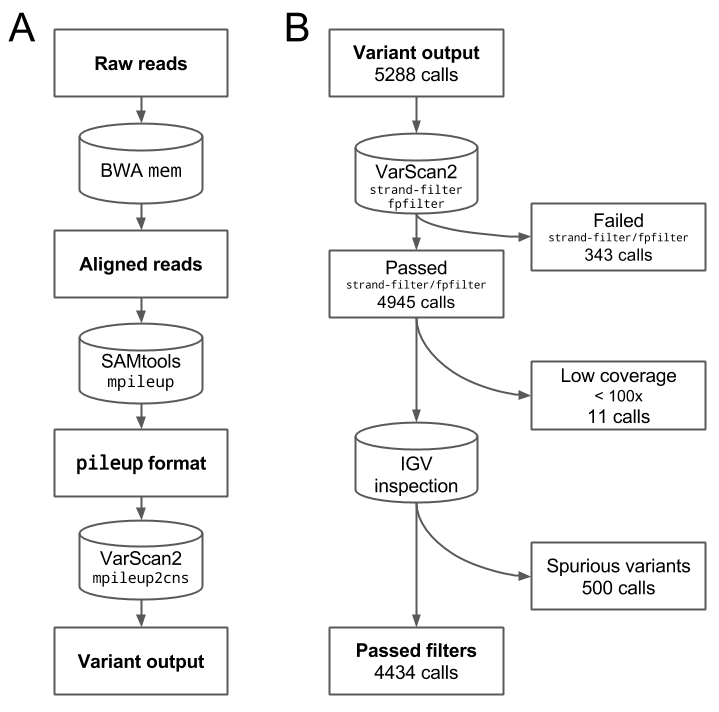
\includegraphics[scale=0.4]{variant_pipeline4.png}
	\caption{Pipelines for (A) variant calling and (B) filtering.}
	\label{variant_pipeline}
\end{figure}

%%%%%%%%%%%%%%%%%%%%%%%%%%%%%%%%%%%%%%%%%%%%%%%%%%%%%%%%%%%%%%%%%%%%%%
\begin{figure}[!h]
	\centering
	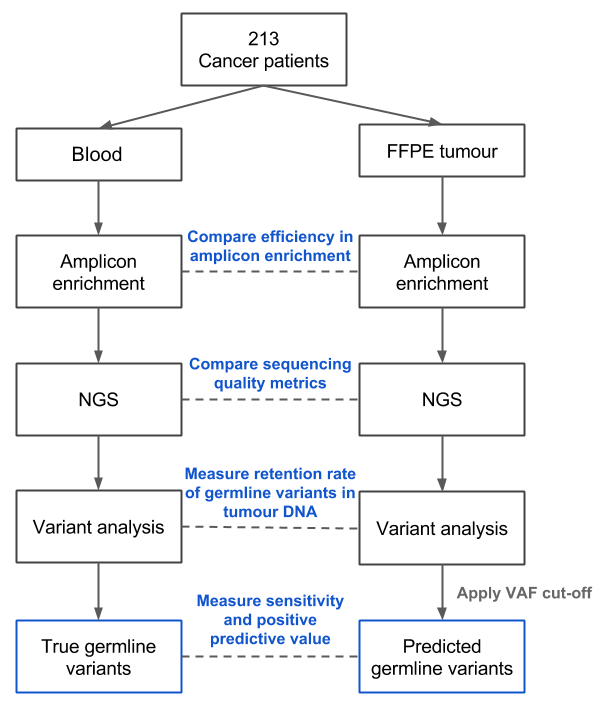
\includegraphics[scale=0.5]{study_design.png}
	\caption{Schematic description of study design and data analyses.}
	\label{study_design}
\end{figure}

%%%%%%%%%%%%%%%%%%%%%%%%%%%%%%%%%%%%%%%%%%%%%%%%%%%%%%%%%%%%%%%%%%%%%%
\begin{figure}[!h]
	\centering
	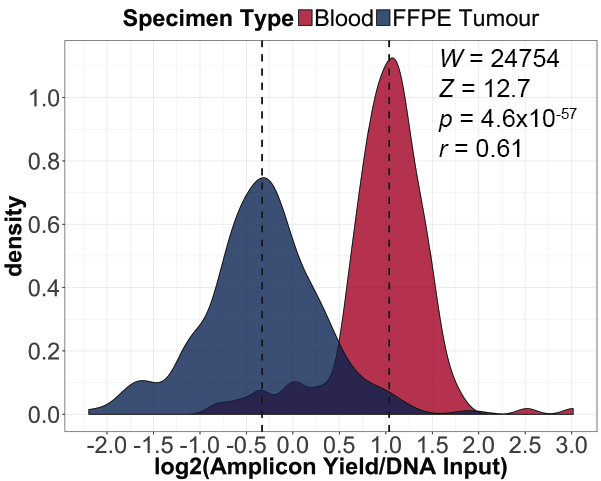
\includegraphics[scale=0.75]{dna_input_amp_yield_xlabel_c.png}
	\caption{Distributions of fold change between DNA input and amplicon yield (log\textsubscript{2}), which is used to measure efficiency in amplicon enrichment in blood and FFPE specimens (Wilcoxon signed-rank test). Dashed lines indicate median log\textsubscript{2} fold change in blood and FFPE specimens, which are 1.04 and -0.332, respectively.}
	\label{dna_input_amp_yield}
\end{figure}

%%%%%%%%%%%%%%%%%%%%%%%%%%%%%%%%%%%%%%%%%%%%%%%%%%%%%%%%%%%%%%%%%%%%%%
\begin{figure}[!h]
\centering
  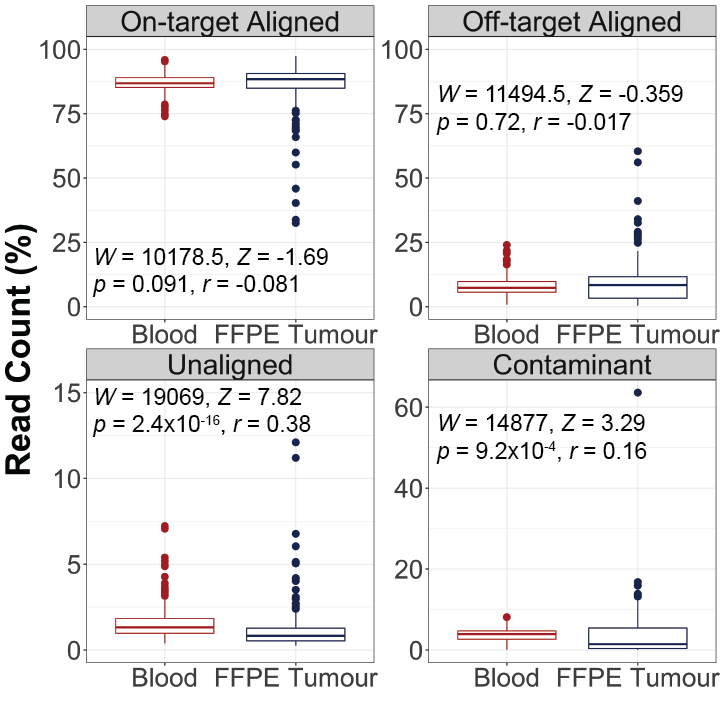
\includegraphics[scale=0.8]{alignment_pct.png}
  \caption[Assessment of read alignments between blood and FFPE specimens (Wilcoxon signed-rank test).]{Assessment of read alignments between blood and FFPE specimens (Wilcoxon signed-rank test). Box plots show the median (horizontal bar within) and interquartile range (IQR) of percentage of reads, with whiskers representing the range of data $\leq$ 1.5x the IQR and circles indicating outliers.}
  \label{alignment_pct}
\end{figure}

%%%%%%%%%%%%%%%%%%%%%%%%%%%%%%%%%%%%%%%%%%%%%%%%%%%%%%%%%%%%%%%%%%%%%%
\begin{figure}[!h]
\centering
  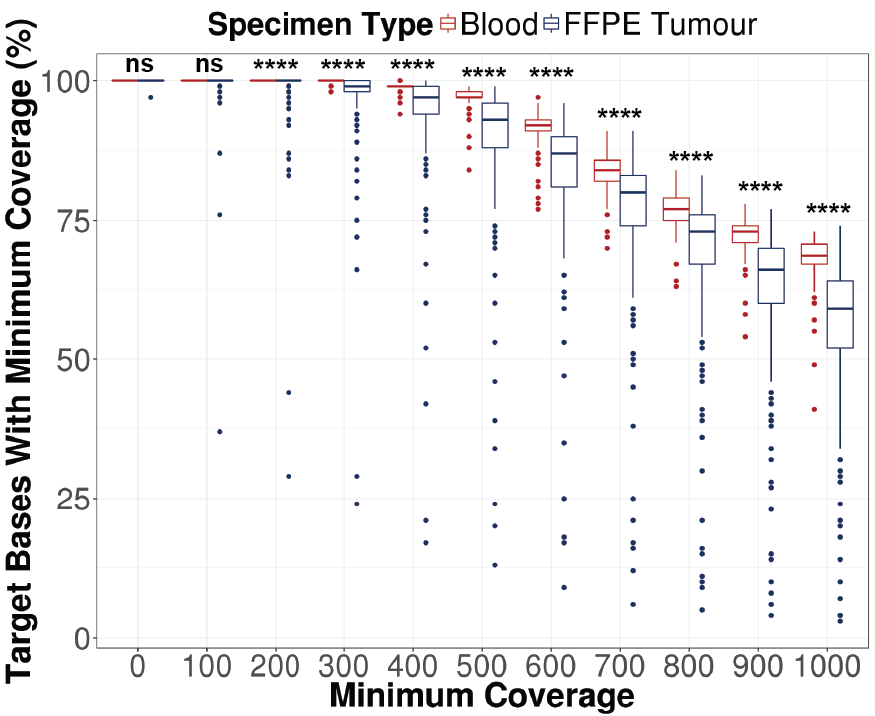
\includegraphics[scale=0.7]{coverage_stats.png}
  \caption[Evaluation of coverage uniformity in blood and FFPE specimens (Wilcoxon signed-rank test, ****\textit{p} $<$ 0.0001, ns = not significant).]{Evaluation of coverage uniformity in blood and FFPE specimens (Wilcoxon signed-rank test, ****\textit{p} $<$ 0.0001, ns = not significant). Per base coverage was normalized to account for difference in library size. Percentage of target bases that met various coverage thresholds was calculated. Box plots show the median (horizontal bar within) and IQR of percentage of target bases that met the respective coverage thresholds, with whiskers representing the range of data $\leq$ 1.5x the IQR and circles indicating outliers.}
  \label{coverage_stats}
\end{figure}

%%%%%%%%%%%%%%%%%%%%%%%%%%%%%%%%%%%%%%%%%%%%%%%%%%%%%%%%%%%%%%%%%%%%%%
\begin{figure}[!h]
\centering
  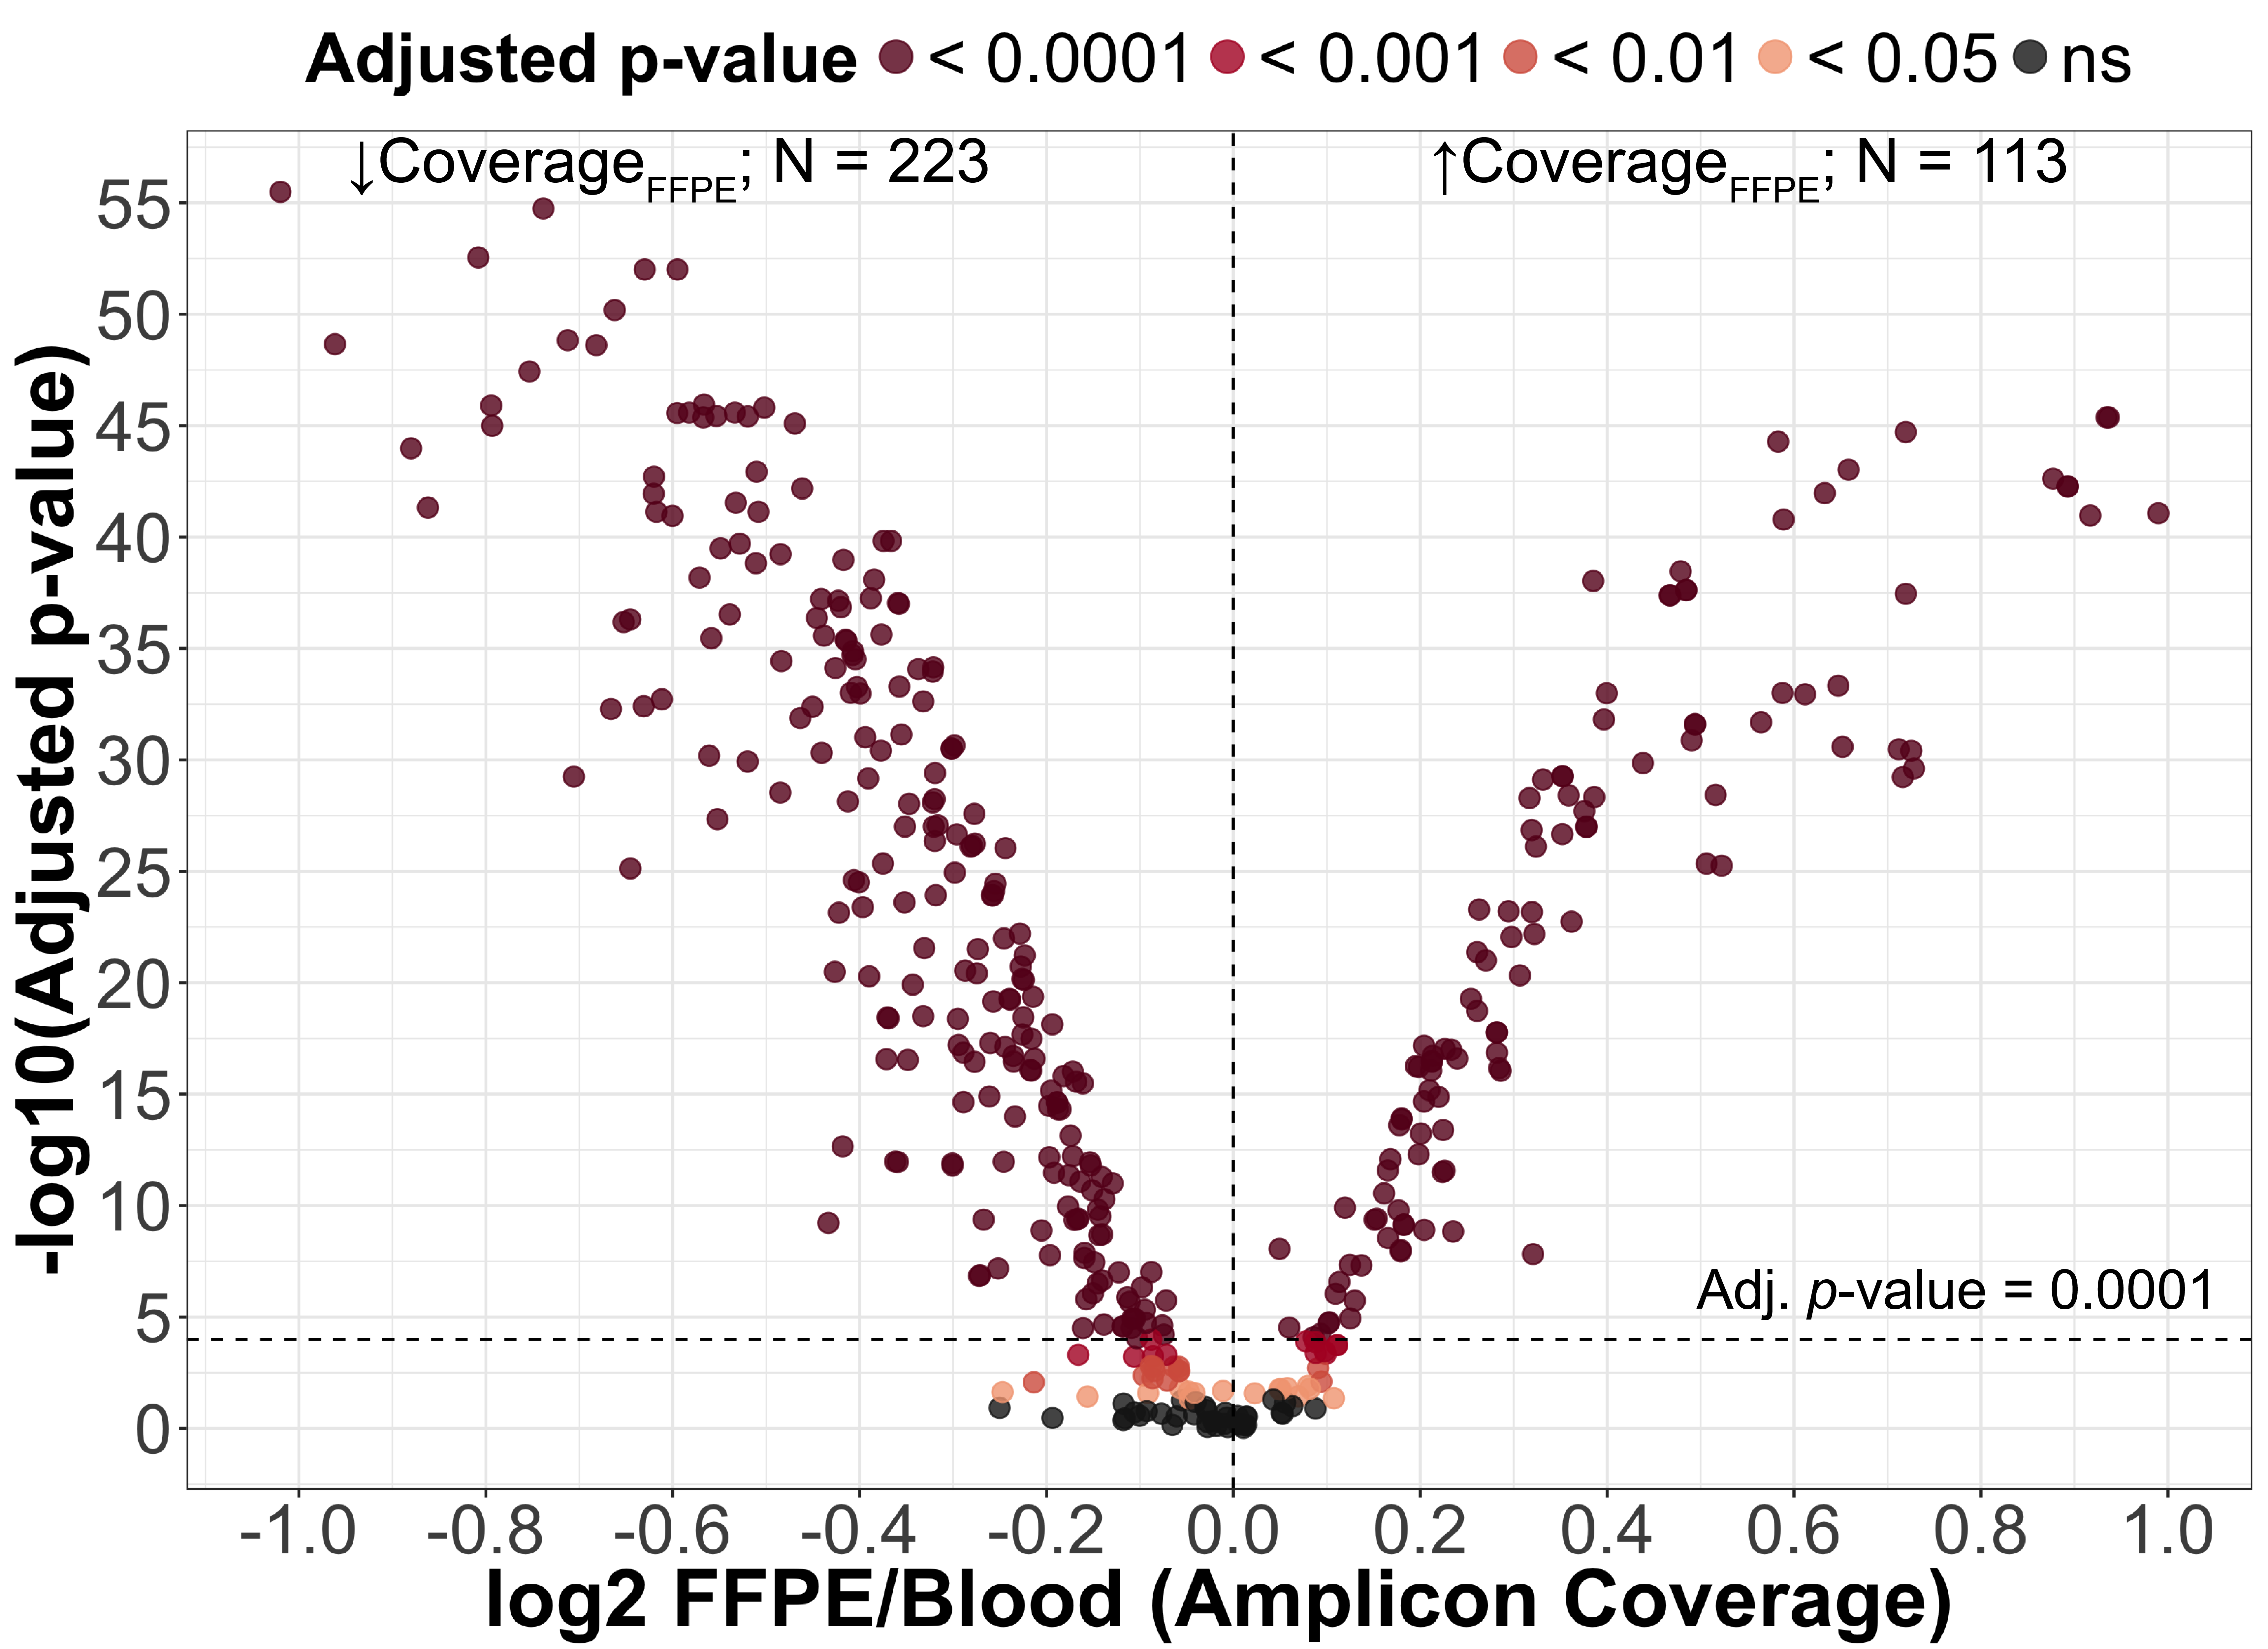
\includegraphics[scale=0.1]{amp_norm_depth_med_wilcoxon_volcano_85_xlabel.png}
  \caption[Amplicon-specific differences in coverage depth between blood and FFPE specimens.]{Amplicon-specific differences in coverage depth between blood and FFPE specimens. Difference in amplicon coverage depth between specimen types was determined using the Wilcoxon signed-rank test with Benjamini-Hochberg correction (adjusted \textit{p} $<$ 0.0001). Volcano plot illustrates the -log\textsubscript{10} adjusted \textit{p}-value in relation to log\textsubscript{2} fold change between median coverage depth in blood and FFPE specimens (\mbox{log\textsubscript{2} (Median Coverage\textsubscript{FFPE}/Median Coverage\textsubscript{Blood})}) for amplicons in the panel. Negative log\textsubscript{2} fold change indicates lower coverage depth of the amplicon in FFPE specimens relative to blood ($\downarrow \text{Coverage\textsubscript{FFPE}}$), whereas positive log\textsubscript{2} fold change indicates higher coverage depth of the amplicon in FFPE specimens relative to blood ($\uparrow\text{Coverage\textsubscript{FFPE}}$). N = number of amplicons; ns = not significant}
  \label{amp_norm_depth_med_wilcoxon_volcano}
\end{figure}

%%%%%%%%%%%%%%%%%%%%%%%%%%%%%%%%%%%%%%%%%%%%%%%%%%%%%%%%%%%%%%%%%%%%%%
\begin{figure}[!h]
	\centering
	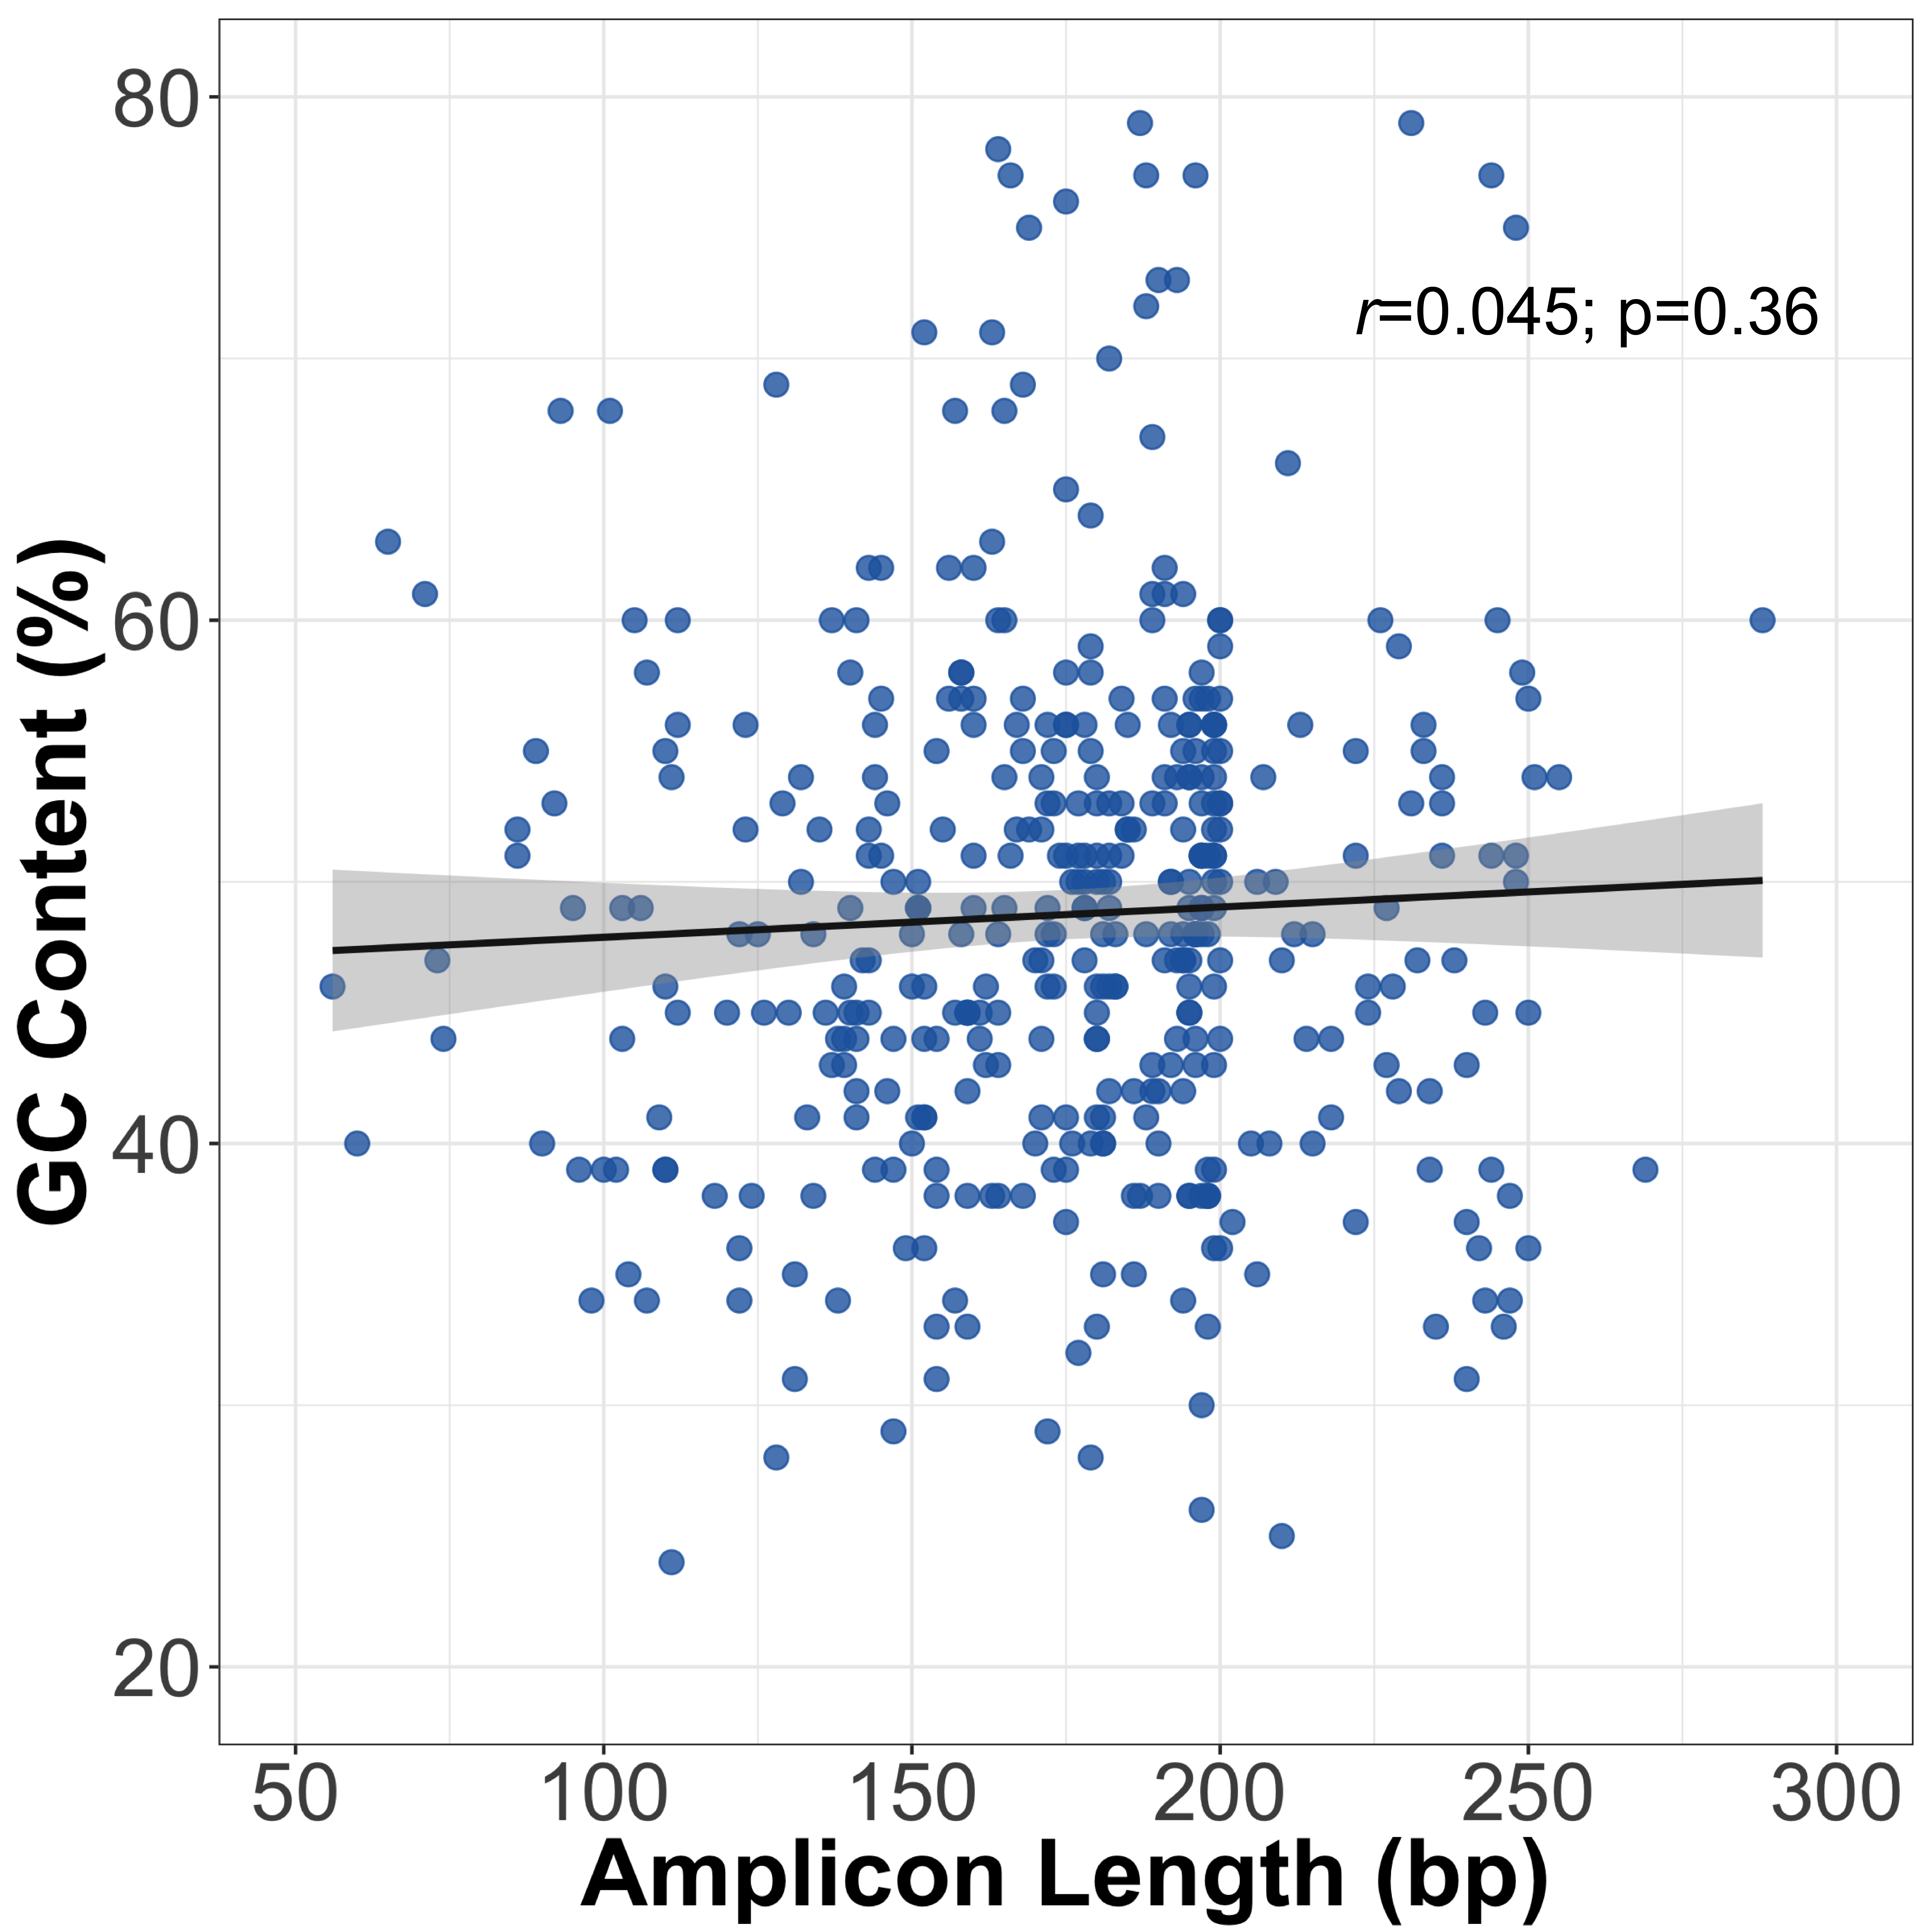
\includegraphics[scale=0.08]{amp_gc_length.png}
	\caption[The relationship between amplicon GC content and amplicon length (Pearson's correlation).]{The relationship between amplicon GC content and amplicon length (Pearson's correlation). Solid line represents the fitted linear relationship between the two variables, and the shaded band indicates pointwise 95\% confidence interval of the fitted linear regression line. (Supplementary)}
	\label{amp_gc_length}
\end{figure}

%%%%%%%%%%%%%%%%%%%%%%%%%%%%%%%%%%%%%%%%%%%%%%%%%%%%%%%%%%%%%%%%%%%%%%
\begin{figure}[!h]
	\centering
  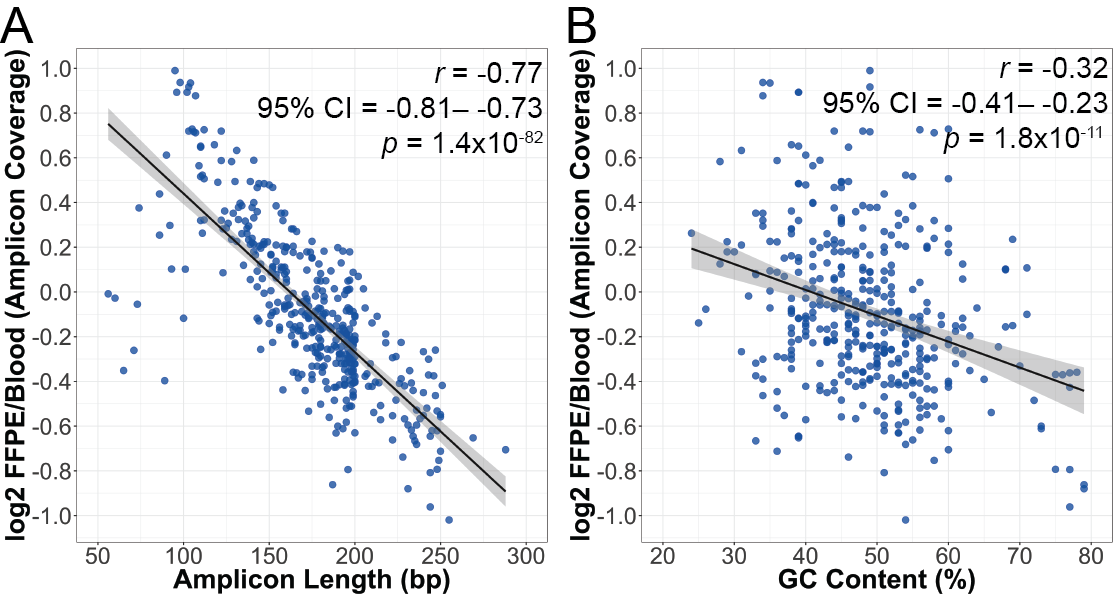
\includegraphics[scale=0.6]{amp_cov_lm_len_gc_85_ylabel.png}
	\caption[Scatter plots showing log\textsubscript{2} fold change between amplicon coverage depth in blood and FFPE specimens in relation to (A) amplicon length and (B) GC content (Pearson's correlation).]{Scatter plots showing log\textsubscript{2} fold change between amplicon coverage depth in blood and FFPE specimens (\mbox{log\textsubscript{2} (Median Coverage\textsubscript{FFPE}/Median Coverage\textsubscript{Blood})}) in relation to (A) amplicon length and (B) GC content (Pearson's correlation). Solid line represents the fitted linear relationship between the two variables, and the shaded band indicates pointwise 95\% confidence interval of the fitted linear regression line.}
	\label{amp_cov_lm_len_gc}
\end{figure}

%%%%%%%%%%%%%%%%%%%%%%%%%%%%%%%%%%%%%%%%%%%%%%%%%%%%%%%%%%%%%%%%%%%%%%
\begin{figure}[!h]
	\centering
	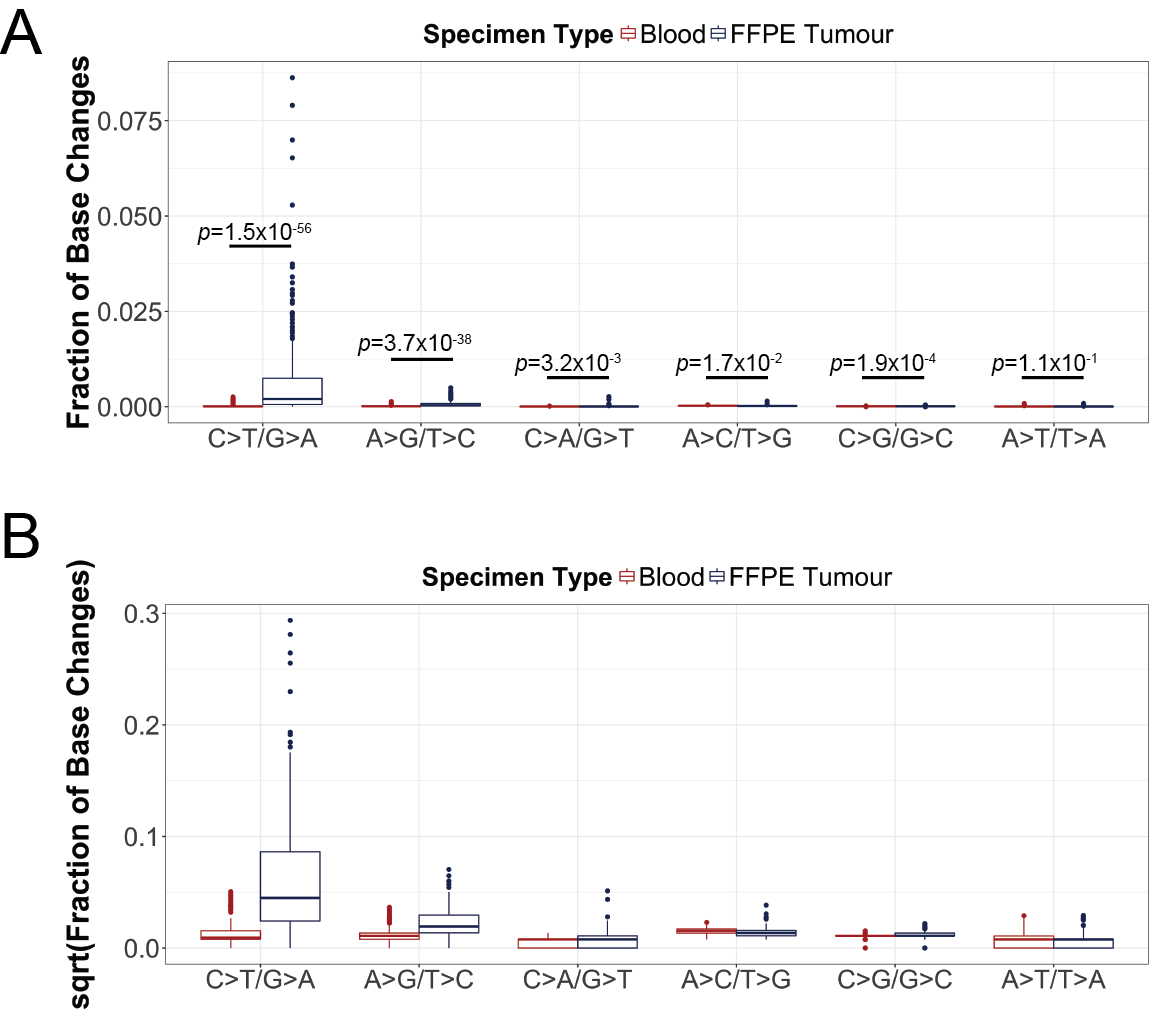
\includegraphics[scale=0.6]{deamination_effect_blood_ffpe.png}
	\caption[Assessment of formalin-induced sequence artifacts in FFPE specimens.]{Assessment of formalin-induced sequence artifacts in FFPE specimens. (A) Comparison of fraction of base changes in blood and FFPE specimens (Wilcoxon signed-rank test). Box plots show the median (horizontal bar within) and IQR of fraction of base changes for different types of base changes, with whiskers representing the range of data $\leq$ 1.5x the IQR and circles indicating outliers. (B) Box plots showing square root-transformed fraction of base changes on the Y-axis.}
	\label{deamination_effect_blood_ffpe}
\end{figure}

%%%%%%%%%%%%%%%%%%%%%%%%%%%%%%%%%%%%%%%%%%%%%%%%%%%%%%%%%%%%%%%%%%%%%%
\begin{figure}[!h]
	\centering
	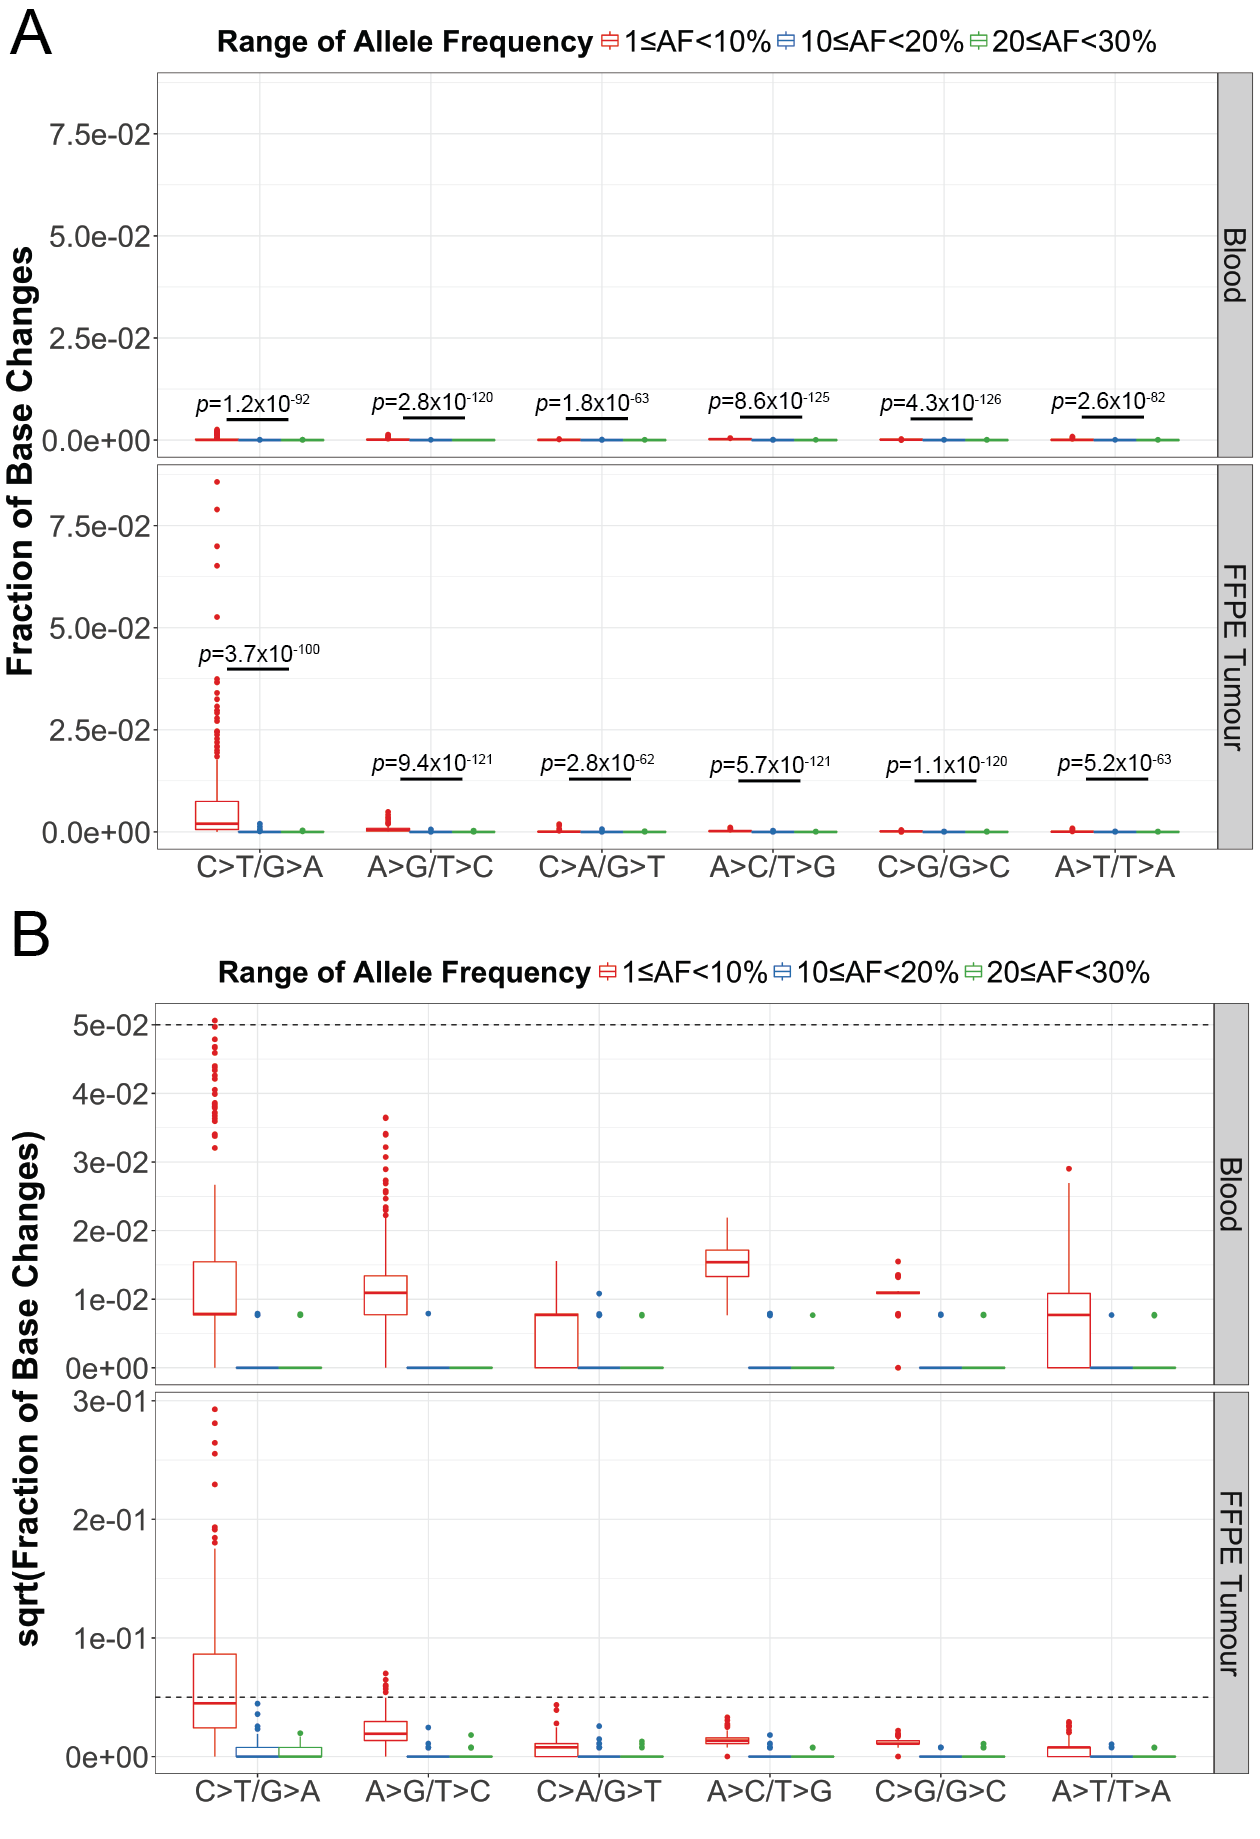
\includegraphics[scale=0.55]{deamination_effect_af_range_2.png}
  \caption[Assessment of formalin-induced sequence artifacts in FFPE specimens at different ranges of allele frequency.]{Assessment of formalin-induced sequence artifacts in FFPE specimens at different ranges of allele frequency. (A) Comparison of fraction of base changes across different ranges of allele frequency (Kruskal-Wallis test). Box plots show the median (horizontal bar within) and IQR of fraction of base changes for different types of base changes, with whiskers representing the range of data $\leq$ 1.5x the IQR and circles indicating outliers. (B) Box plots demonstrating square root-transformed fraction of base changes across different ranges of allele frequency. Dashed lines equal to 0.05 to indicate that the Y-axis scales are different for blood and FFPE tumour plots.}
	\label{deamination_effect_af_range}
\end{figure}

%%%%%%%%%%%%%%%%%%%%%%%%%%%%%%%%%%%%%%%%%%%%%%%%%%%%%%%%%%%%%%%%%%%%%%
\begin{figure}[!h]
	\centering
	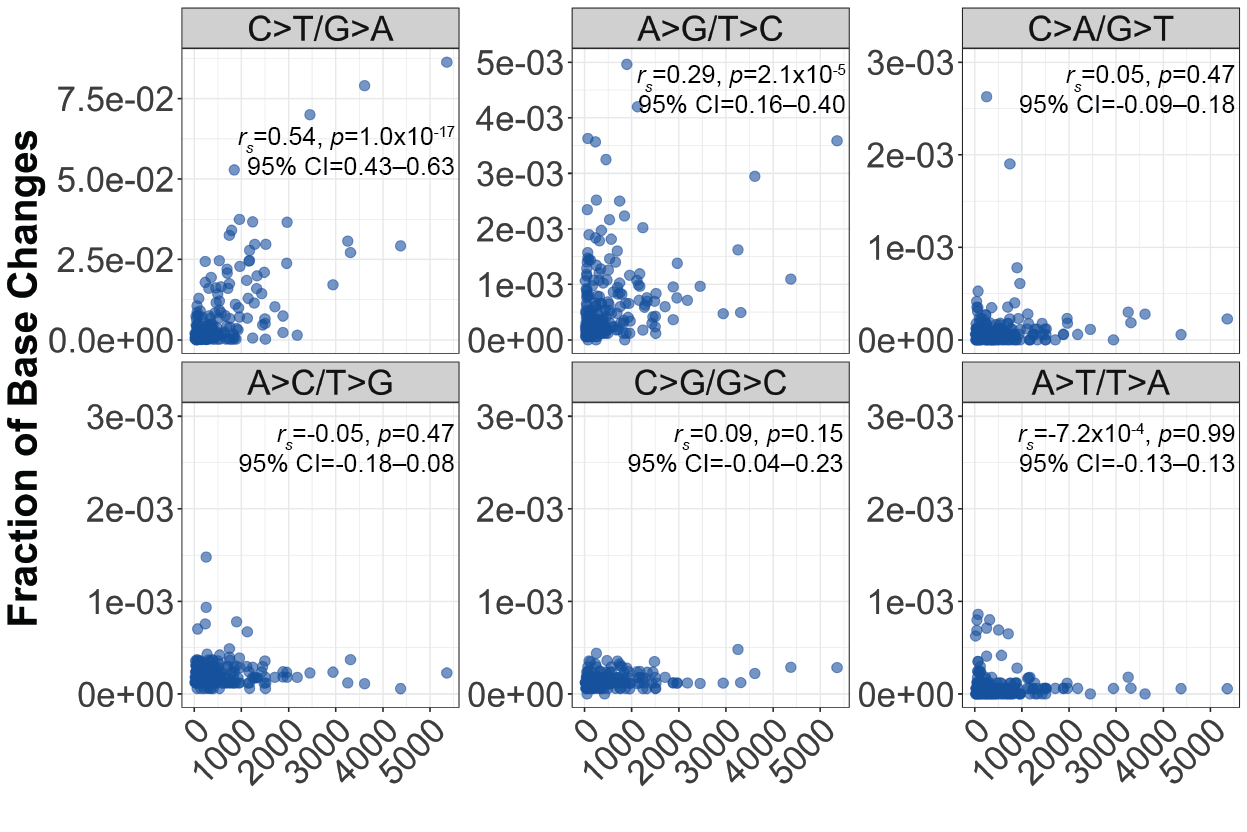
\includegraphics[scale=0.55]{deamination_effect_age.png}
	\caption{The relationship between fraction of base changes and age of paraffin block for different types of base changes (Spearman's rank correlation).}
	\label{deamination_effect_age}
\end{figure}

%%%%%%%%%%%%%%%%%%%%%%%%%%%%%%%%%%%%%%%%%%%%%%%%%%%%%%%%%%%%%%%%%%%%%%
\begin{figure}[!h]
\centering
	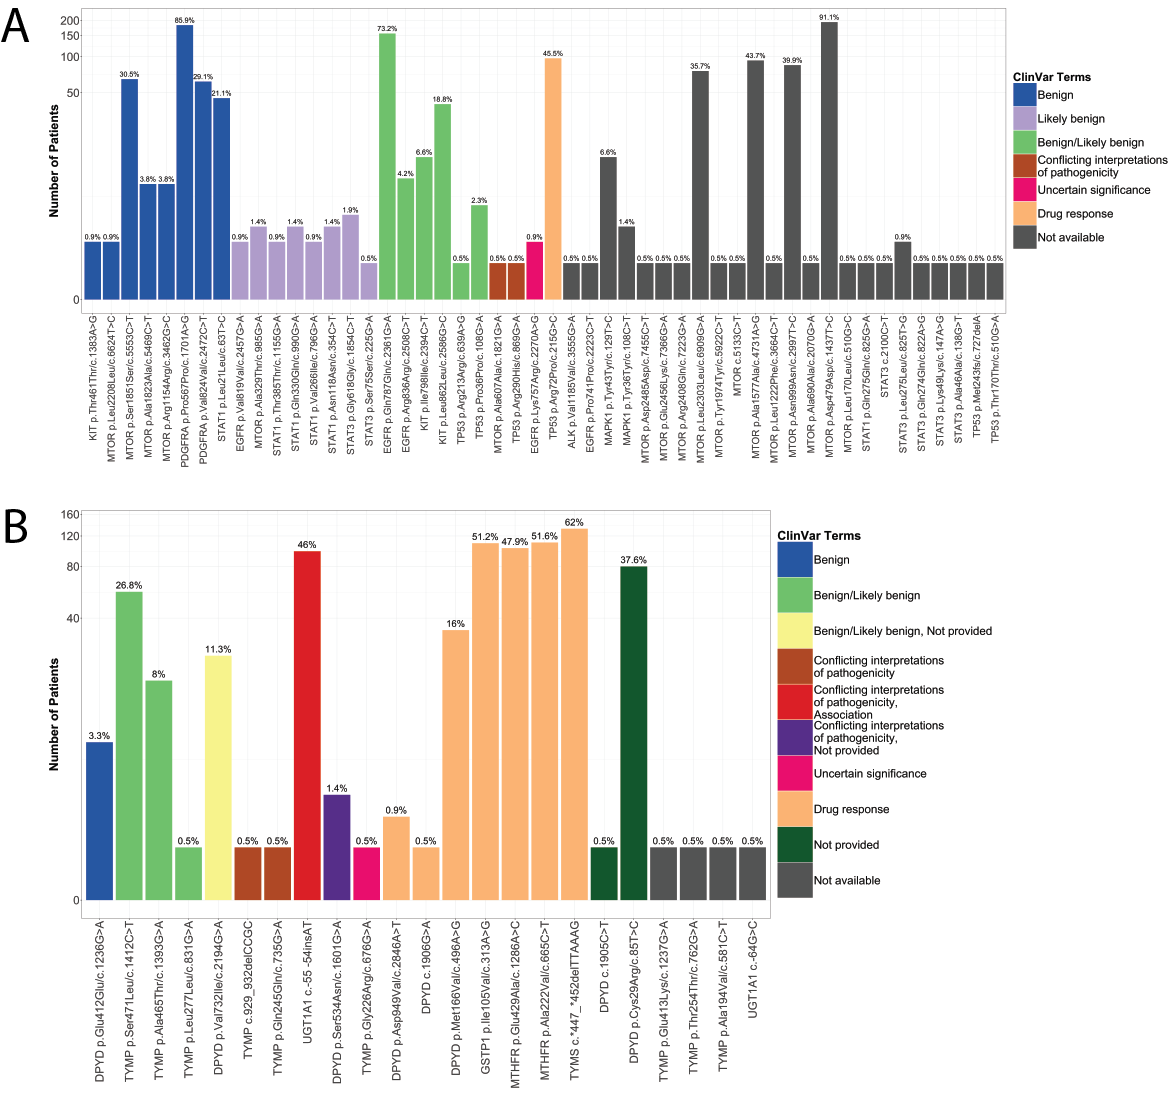
\includegraphics[scale=0.63]{bar_pct.png}
	\caption{Distribution of germline alterations in (A) cancer-related and (B) PGx genes in patients from TOP study. Percentage of patients is calculated for each variant and annotated above individual bars. Color of bars represent options for clinical significance in the ClinVar database. log(1 + x) transformation is applied to change the scale of set values on the Y-axis.}
	\label{bar_pct}
\end{figure}

%%%%%%%%%%%%%%%%%%%%%%%%%%%%%%%%%%%%%%%%%%%%%%%%%%%%%%%%%%%%%%%%%%%%%%
\begin{figure}[!h]
\centering
	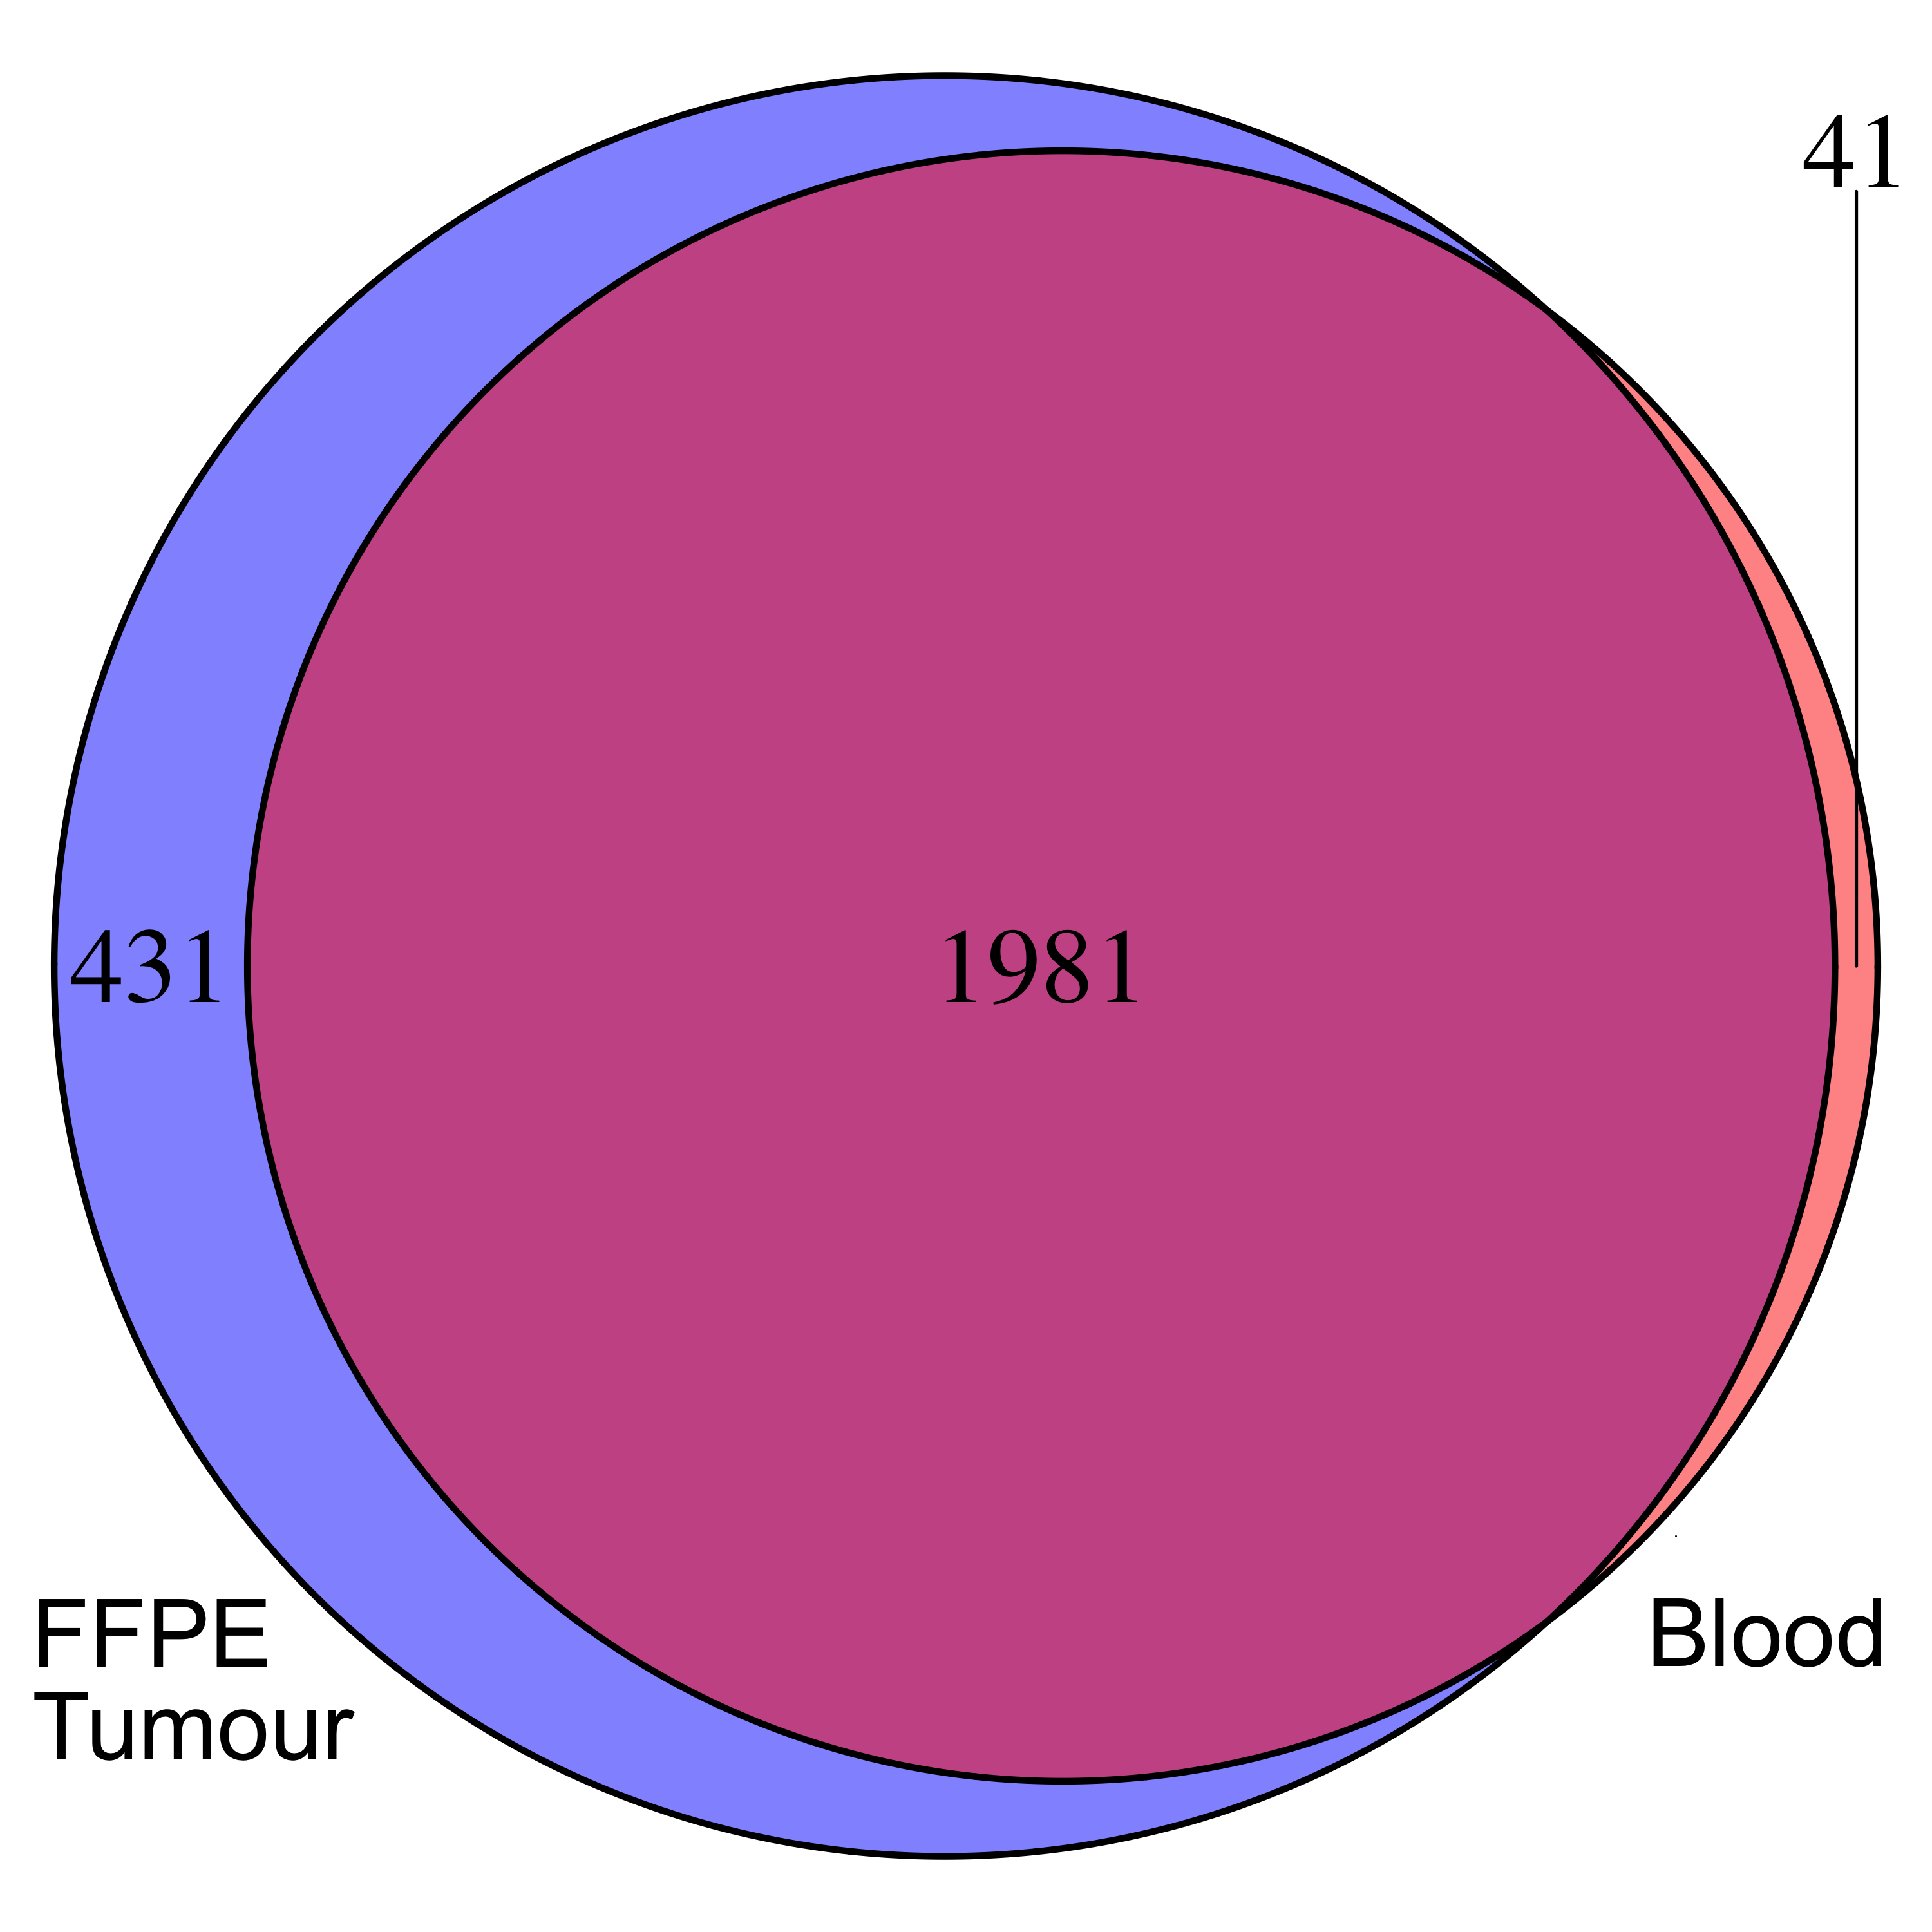
\includegraphics[scale=0.06]{ffpe_blood_conc_venn.png}
	\caption{Venn diagram demonstrating concordance of variants identified in 217 tumour-blood paired samples.}
	\label{ffpe_blood_conc_venn}
\end{figure}

%%%%%%%%%%%%%%%%%%%%%%%%%%%%%%%%%%%%%%%%%%%%%%%%%%%%%%%%%%%%%%%%%%%%%%
\begin{figure}[!h]
	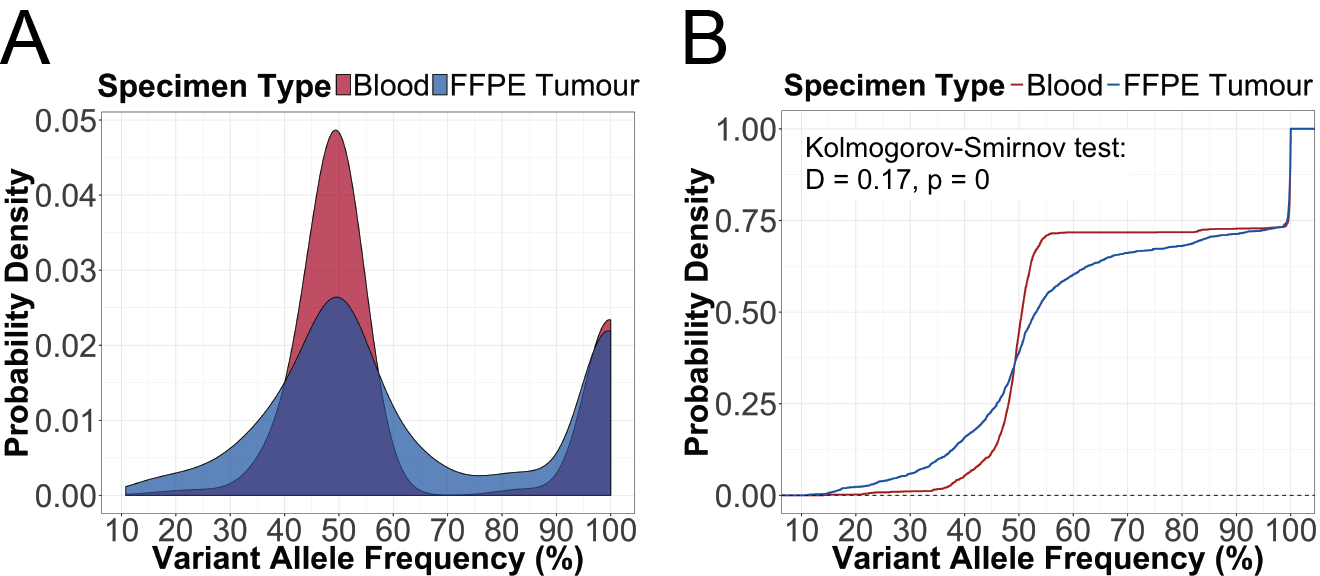
\includegraphics[scale=0.55]{germline_sens_minor_no_line.png}
	\caption[Assessment of using a VAF cut-off approach to identify germline alterations in tumour-only analyses.]{Assessment of using a VAF cut-off approach to identify germline alterations in tumour-only analyses. (A) Comparison of VAF distributions of germline alterations between blood and tumour. (B) Empirical cumulative distribution of VAFs of germline alterations in blood and tumour samples (Kolmogorov-Smirnov test).}
	\label{germline_sens_minor}
\end{figure}

%%%%%%%%%%%%%%%%%%%%%%%%%%%%%%%%%%%%%%%%%%%%%%%%%%%%%%%%%%%%%%%%%%%%%%

\begin{figure}[!h]
	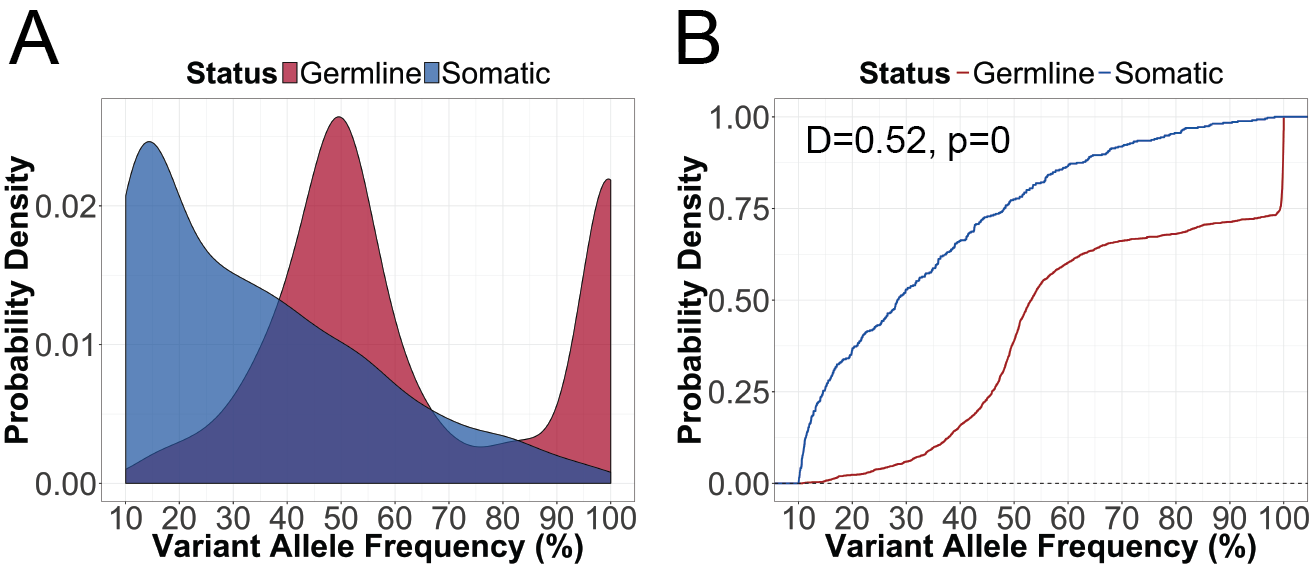
\includegraphics[scale=0.55]{germline_ppv_minor_no_line.png}
	\caption[Assessment of using a VAF cut-off approach to refer potential germline alterations in tumour-only analyses to follow-up testing.]{Assessment of using a VAF cut-off approach to refer potential germline alterations in tumour-only analyses to follow-up testing. (A) Comparison of VAF distributions between germline and somatic alterations in tumour specimens. (B) Empirical cumulative distribution of VAFs of germline and somatic alterations in tumour samples (Kolmogorov-Smirnov test).}
	\label{germline_ppv_minor}
\end{figure}

\FloatBarrier

%%%%%%%%%%%%%%%%%%%%%%%%%%%%%%%%%%%%%%%%%%%%%%%%%%%%%%%%%%%%%%%%%%%%%%


%%%%%%%%%%%%%%%%%%%%%%%%%%%%%%%%%%%
%%                               %%
%% Tables                        %%
%%                               %%
%%%%%%%%%%%%%%%%%%%%%%%%%%%%%%%%%%%

%% Use of \listoftables is discouraged.
%%
\section*{Tables}

%%%%%%%%%%%%%%%%%%%%%%%%%%%%%%%%%%%%%%%%%%%%%%%%%%%%%%%%%%%%%%%%%%%%%%
\begin{table}[H]
\caption{Distribution of cancer types in the TOP cohort.}
\label{cancertypes}
\centering
      \begin{tabular}{lccc}
        \hline
        Cancer Type & Number of Cases & Percentage (\%) \\ \hline
        Colorectal & 97 & 46 \\
        Lung & 60 & 28 \\
        Melanoma & 18 & 8 \\
				Other\textsuperscript{$\dagger$} & 16 & 8 \\
				GIST & 7 & 3 \\
				Sarcoma & 4 & 2 \\
				Neuroendocrine & 4 & 2 \\
				Cervical & 2 & 0.9 \\
				Ovarian & 2 & 0.9 \\
				Breast & 2 & 0.9 \\
				Unknown & 1 & 0.5 \\ \hline
      \end{tabular} \\
			\vspace{0.3cm}
\justify
\textsuperscript{$\dagger$}This category includes thyroid, peritoneum, Fallopian tube, gastric, endometrial, squamous cell carcinoma, anal, salivary gland, peritoneal epithelial mesothelioma, adenoid cystic carcinoma, pancreas, breast, gall bladder, parotid epithelial myoepithelial carcinoma, carcinoid, and small bowel cancers.
\end{table}

%%%%%%%%%%%%%%%%%%%%%%%%%%%%%%%%%%%%%%%%%%%%%%%%%%%%%%%%%%%%%%%%%%%%%%
\begin{table}[H]
\caption{Gene reference models for HGVS nomenclature of OncoPanel genes.}
\label{tbl:genemodel}
    \centering
    \begin{tabular}{llll}
    \hline
    Gene & Protein & Reference Model \\
    \hline
    \multicolumn{3}{l}{\textit{Cancer-related}}
    \\
    AKT1 & Protein kinase B & NM\_001014431.1 \\
    ALK & Anaplastic lymphoma receptor tyrosine kinase & NM\_004304.3 \\
    BRAF & Serine/threonine-protein kinase B-Raf & NM\_004333.4 \\
    EGFR & Epidermal growth factor receptor & NM\_005228.3 \\
    HRAS & GTPase HRas & NM\_005343.2 \\
    MAPK1 & Mitogen-activated protein kinase 1 & NM\_002745.4 \\
    MAP2K1 & Mitogen-activated protein kinase kinase 1 & NM\_002755.3 \\
    MTOR & Serine/threonine-protein kinase mTOR & NM\_004958.3 \\
    NRAS & Neuroblastoma RAS viral oncogene homolog & NM\_002524.3 \\
    PDGFRA & Platelet-derived growth factor receptor alpha & NM\_006206.4 \\
    PIK3CA & Phosphatidylinositol-4,5-bisphosphate 3-kinase catalytic subunit alpha & NM\_006218.2 \\
    PTEN & Phosphatase and tensin homolog & NM\_000314.4 \\
    STAT1 & Signal transducer and activator of transcription 1 & NM\_007315.3 \\
    STAT3 & Signal transducer and activator of transcription 3 & NM\_139276.2 \\
    TP53 & Tumor protein P53 & NM\_000546.5 \\
    \\
    \multicolumn{3}{l}{\textit{Pharmacogenomic-related}}
    \\
    DPYD & Dihydropyrimidine dehydrogenase & NM\_000110.3 \\
    GSTP1 & Glutathione S-rransferase pi 1 & NM\_000852.3 \\
    MTHFR & Methylenetetrahydrofolate reductase & NM\_005957.4 \\
    TYMP & Thymidine phosphorylase & NM\_001113755.2 \\
    TYMS & Thymidylate synthetase & NM\_001071.2 \\
    UGT1A1 & Uridine diphosphate (UDP)-glucuronosyl transferase 1A1 & NM\_000463.2\\
    \hline
    \end{tabular}
\end{table}

%%%%%%%%%%%%%%%%%%%%%%%%%%%%%%%%%%%%%%%%%%%%%%%%%%%%%%%%%%%%%%%%%%%%%%
\begin{longtable}{p{0.08\linewidth}|p{0.05\linewidth}p{0.1\linewidth}p{0.13\linewidth}p{0.16\linewidth}p{0.2\linewidth}}
    \caption{Potential minor alleles in the hg19 human reference genome within the target regions of the OncoPanel. (Supplementary)}
    \label{potential_risk_alleles}
        \\
        \hline
        Gene & Chr & Pos & Minor Allele & dbSNP ID & HGVS\textsuperscript{*}
				\\
				\hline
        DPYD & chr1 & 98348885 & C & rs1801265 & p.Cys29Arg c.85T$>$C
        \\
        MTOR & chr1 & 11205058 & G & rs386514433; rs1057079 & p.Ala1577Ala c.4731A$>$G
        \\
        & chr1 & 11288758 & C & rs1064261 & p.Asn999Asn c.2997T$>$C
        \\
        TP53 & chr17 & 7579472 & C & rs1042522 & p.Arg72Pro c.215G$>$C
        \\
				\hline
        \caption*{\textsuperscript{*}Description of sequence variants according to the HGVS recommendations.}
\end{longtable}

%%%%%%%%%%%%%%%%%%%%%%%%%%%%%%%%%%%%%%%%%%%%%%%%%%%%%%%%%%%%%%%%%%%%%%
\begin{table}[H]
\caption{Thresholds for parameters of VarScan2 \texttt{fpfilter} used for filtering raw variant output. (Supplementary)}
\label{varscan_fpfilter_parameters}
\centering
      \begin{tabular}{p{0.3\linewidth}p{0.56\linewidth}cp{0.1\linewidth}}
        \hline
        Parameter & Description & Threshold
				\\
				\hline
				\texttt{--min-var-count} & Min number of var-supporting reads & 4
				\\
        \texttt{--min-var-count-lc} & Min number of var-supporting reads when depth below somaticPdepth & 2
        \\
        \texttt{--min-var-freq} & Min variant allele frequency & 0.1
				\\
        \texttt{--max-somatic-p} & Max somatic p-value & 0.05
				\\
        \texttt{--max-somatic-p-depth} & Depth required to test max somatic p-value & 10
				\\
        \texttt{--min-ref-readpos} & Min average read position of ref-supporting reads & 0.1
				\\
        \texttt{--min-var-readpos} & Min average read position of var-supporting reads & 0.1
				\\
        \texttt{--min-ref-dist3} & Min average distance to effective 3' end of ref reads & 0.1
				\\
        \texttt{--min-var-dist3} & Min average distance to effective 3' end of variant reads & 0.1
				\\
        \texttt{--min-strandedness} & Min fraction of variant reads from each strand & 0.1
				\\
        \texttt{--min-strand-reads} & Min allele depth required to perform the strand tests & 5
				\\
        \texttt{--min-ref-basequal} & Min average base quality for ref allele & 15
				\\
        \texttt{--min-var-basequal} & Min average base quality for var allele & 15
				\\
        \texttt{--min-ref-avgrl} & Min average trimmed read length for ref allele & 90
				\\
        \texttt{--min-var-avgrl} & Min average trimmed read length for var allele & 90
        \\
        \texttt{--max-rl-diff} & Max average relative read length difference (ref - var) & 0.25
        \\
        \texttt{--max-ref-mmqs} & Max mismatch quality sum of ref-supporting reads & 100
        \\
        \texttt{--max-var-mmqs} & Max mismatch quality sum of var-supporting reads & 100
        \\
        \texttt{--max-mmqs-diff} & Max average mismatch quality sum (var - ref) & 50
        \\
        \texttt{--min-ref-mapqual} & Min average mapping quality for ref allele & 15
        \\
        \texttt{--min-var-mapqual} & Min average mapping quality for var allele & 15
        \\
        \texttt{--max-mapqual-diff} & Max average mapping quality (ref - var) & 50
        \\
				\hline
      \end{tabular}
\end{table}

%%%%%%%%%%%%%%%%%%%%%%%%%%%%%%%%%%%%%%%%%%%%%%%%%%%%%%%%%%%%%%%%%%%%%%
\begin{longtable}{p{0.08\linewidth}p{0.05\linewidth}p{0.1\linewidth}p{0.04\linewidth}p{0.04\linewidth}p{0.4\linewidth}}
    \caption{Spurious variants removed by the variant filtering pipeline. (Supplementary)}
    \label{spurious_calls}
        \\
        \hline
        Gene & Chr & Pos & Ref & Alt & Reason
				\\
				\hline
				KIT & chr4 & 55599268 & C & T & Variant masked by primer in FFPE specimen
				\\
        MAPK1 & chr22 & 22162126 & A & G & Variant masked by primer in FFPE specimen
        \\
        MTOR & chr1 & 11186783 & G & A & Sequencing artifact within primer region
        \\
        MTOR & chr1 & 11190646 & G & A & Variant masked by primer in FFPE specimen
        \\
        TYMP & chr22 & 50964446 & A & T & Poor target region, alignment of different sized amplicons
        \\
        TYMP & chr22 & 50964862 & A & T & Poor target region, alignment of different sized amplicons
        \\
        TYMS & chr18 & 673449 & G & C & VarScan2 bug after chr18:673443 c.*447\_*452delTTAAAG
        \\
        UGT1A1 & chr2 & 234668879 & CAT & C & Sequencing artifact at AT repeats in promoter
        \\
        UGT1A1 & chr2 & 234668881 & T & TAC & VarScan2 bug after AT insertion in promoter
        \\
				\hline
\end{longtable}

%%%%%%%%%%%%%%%%%%%%%%%%%%%%%%%%%%%%%%%%%%%%%%%%%%%%%%%%%%%%%%%%%%%%%%
\begin{table}[H]
\caption[Multiple linear regression to predict log\textsubscript{2} fold change between amplicon coverage depth in blood and FFPE specimens based on amplicon length and GC content.]{Multiple linear regression to predict log\textsubscript{2} fold change between amplicon coverage depth in blood and FFPE specimens (\mbox{log\textsubscript{2} (Median Coverage\textsubscript{FFPE}/Median Coverage\textsubscript{Blood})}) based on amplicon length and GC content.}
\label{multiple_regression}
\centering
      \begin{tabular}{l|ccccl}
        Variable & Unstandardized Coefficient & Standard Error & Standardized Coefficient & \textit{p}-value
        \\
        \hline
        Length (bp) & \num{-6.97e-3} & \num{2.59e-4} & \num{-7.56e-1} & \num{7.45e-93}
				\\
				GC Content (\%) & \num{-1.03e-2} & \num{1.01e-3} & \num{-2.88e-1} & \num{4.71e-22}
				\\
				\hline
				\\
				 & \multicolumn{4}{r}{Intercept = 1.63, Adjusted R\textsuperscript{2} = 0.673}
				\\
				 & \multicolumn{4}{r}{\textit{F}(2, 413) = 427.6, \textit{p}-value = \num{2.41e-101}}
				\\
				\hline
      \end{tabular} \\
\end{table}

%%%%%%%%%%%%%%%%%%%%%%%%%%%%%%%%%%%%%%%%%%%%%%%%%%%%%%%%%%%%%%%%%%%%%%
\begin{table}[H]
\caption{Comparison of coverage uniformity between blood and FFPE specimens using the Wilcoxon signed-rank test. (Supplementary)}
\label{coverage_uniformity}
\centering
      \begin{tabular}{llllllcll}
        \hline
				\multicolumn{1}{l}{ }
				&
				\multicolumn{2}{l}{Blood}
				&&
				\multicolumn{2}{l}{FFPE Tumour}
				&
				\multicolumn{2}{l}{ } \\
				\cline{2-3}\cline{5-6}
        Threshold & Median (\%) & Range (\%) && Median (\%) & Range (\%) & \textit{D}\textsuperscript{$\dagger$} (\%) & \textit{p} ($<$ 0.0001\textsuperscript{*})
				\\
				\hline
				$\geq$ 0x & 100 & 100--100 && 100 & 97.0--100 & 0.0 & 1.0
				\\
				$\geq$ 100x & 100 & 100--100 && 100 & 37.0--100 & 0.0 & \num{2.3e-4}
				\\
				$\geq$ 200x & 100 & 100--100 && 100 & 29.0--100 & 0.0 & \num{2.9e-11}\textsuperscript{*}
				\\
				$\geq$ 300x & 100 & 98.0--100 && 99.0 & 24.0--100 & 1.0 & \num{4.1e-18}\textsuperscript{*}
				\\
				$\geq$ 400x & 99.0 & 94.0--100 && 97.0 & 17.0--100 & 2.0 & \num{5.0e-28}\textsuperscript{*}
				\\
				$\geq$ 500x & 97.0 & 84.0--99.0 && 89.5 & 13.0--99.0 & 7.5 & \num{2.1e-38}\textsuperscript{*}
				\\
				$\geq$ 600x & 92.0 & 77.0--97.0 && 87.0 & 9.0--96.0 & 5.0 & \num{1.5e-32}\textsuperscript{*}
				\\
				$\geq$ 700x & 84.0 & 70.0--91.0 && 80.0 & 6.0--91.0 & 4.0 & \num{5.7e-25}\textsuperscript{*}
				\\
				$\geq$ 800x & 77.0 & 63.0-84.0 && 73.0 & 5.0--83.0 & 4.0 &  \num{4.7e-27}\textsuperscript{*}
				\\
				$\geq$ 900x & 73.0 & 54.0--78.0 && 66.0 & 4.0--77.0 & 7.0 &  \num{4.6e-40}\textsuperscript{*}
				\\
				$\geq$ 1000x & 68.5 & 41.0--73.0 && 59.0 & 3.0-74.0 & 9.5 &  \num{3.6e-42}\textsuperscript{*}
				\\
				\hline
      \end{tabular}
			\vspace{0.3cm}
      \justify
			\textsuperscript{$\dagger$}Absolute difference between median of blood and FFPE specimens.
\end{table}

%%%%%%%%%%%%%%%%%%%%%%%%%%%%%%%%%%%%%%%%%%%%%%%%%%%%%%%%%%%%%%%%%%%%%%
\begin{table}[H]
\caption{Summary statistics of fraction of base changes in blood and FFPE specimens. (Supplementary)}
\label{sum_stats_base_changes}
\centering
      \begin{tabular}{llllllcl}
        \hline
				\multicolumn{1}{l}{ }
				&
				\multicolumn{2}{l}{Blood}
				&&
				\multicolumn{2}{l}{FFPE Tumour}
				&
				\multicolumn{1}{l}{ } \\
				\cline{2-3}\cline{5-6}
        Base Changes & Median & Range && Median & Range & FC\textsuperscript{$\dagger$}
				\\
				\hline
				C$>$T/G$>$A & \num{8.9e-5} & \num{0}--\num{2.6e-3} && \num{2.0e-3} & \num{0}--\num{8.6e-2} & 23
				\\
				A$>$G/T$>$C & \num{1.2e-4} & \num{0}--\num{1.3e-3} && \num{3.7e-4} & \num{0}--\num{5.0e-3} & 3.1
				\\
				C$>$A/G$>$T & \num{6.0e-5} & \num{0}--\num{1.8e-4} && \num{6.0e-5} & \num{0}--\num{2.6e-3} & 1.0
				\\
				A$>$C/T$>$G & \num{2.4e-4} & \num{5.9e-5}--\num{5.3e-4} && \num{1.8e-4} & \num{5.8e-5}--\num{1.4e-3} & 0.77
				\\
				C$>$G/G$>$C & \num{1.2e-4} & \num{0}--\num{2.4e-4} && \num{1.2e-4} & \num{0}--\num{4.8e-4} & 1.0
				\\
				A$>$T/T$>$A & \num{6.0e-5} & \num{0}--\num{8.4e-4} && \num{5.9e-5} & \num{0}--\num{8.6e-4} & 0.99
				\\
				\hline
      \end{tabular}
			\justify
			\textsuperscript{$\dagger$}Fold change (FC) between the median of blood and FFPE specimens.
\end{table}

%%%%%%%%%%%%%%%%%%%%%%%%%%%%%%%%%%%%%%%%%%%%%%%%%%%%%%%%%%%%%%%%%%%%%%
\begin{table}[H]
\caption{Summary statistics of fraction of base changes in blood and FFPE specimens within 1-10\% allele frequency. (Supplementary)}
\label{sum_stats_base_changes_range}
\centering
      \begin{tabular}{llllllcl}
        \hline
				\multicolumn{1}{l}{ }
				&
				\multicolumn{2}{l}{Blood}
				&&
				\multicolumn{2}{l}{FFPE Tumour}
				&
				\multicolumn{1}{l}{ } \\
				\cline{2-3}\cline{5-6}
        Base Changes & Median & Range && Median & Range & \textsuperscript{$\dagger$}FC
				\\
				\hline
				C$>$T/G$>$A & \num{6.2e-5} & \num{0}--\num{2.6e-3} && \num{2.0e-3} & \num{0}--\num{8.6e-2} & 33
				\\
				A$>$G/T$>$C & \num{1.2e-4} & \num{0}--\num{1.3e-3} && \num{3.7e-4} & \num{0}--\num{4.9e-3} & 3.1
				\\
				C$>$A/G$>$T & \num{6.0e-5} & \num{0}--\num{2.4e-4} && \num{6.0e-5} & \num{0}--\num{1.9e-3} & 1.0
				\\
				A$>$C/T$>$G & \num{2.4e-4} & \num{5.9e-5}--\num{4.8e-4} && \num{1.8e-4} & \num{0}--\num{1.1e-3} & 0.77
				\\
				C$>$G/G$>$C & \num{1.2e-4} & \num{0}--\num{2.4e-4} && \num{1.2e-4} & \num{0}--\num{4.8e-4} & 1.0
				\\
				A$>$T/T$>$A & \num{6.0e-5} & \num{0}--\num{8.4e-4} && \num{5.9e-5} & \num{0}--\num{8.6e-4} & 0.99
				\\
				\hline
      \end{tabular}
			\justify
			{\small \textsuperscript{$\dagger$}Fold change (FC) between the median of blood and FFPE specimens.}
\end{table}

%%%%%%%%%%%%%%%%%%%%%%%%%%%%%%%%%%%%%%%%%%%%%%%%%%%%%%%%%%%%%%%%%%%%%%
\begin{table}[H]
\caption[Spearman's rank correlation between pre-sequencing variables (e.g. enrichment efficiency and age of paraffin block) and sequencing metrics (e.g. fraction of C$>$T/G$>$A, average per base normalized coverage, and on-target aligned reads).]{Spearman's rank correlation between pre-sequencing variables (e.g. enrichment efficiency and age of paraffin block) and sequencing metrics (e.g. fraction of C$>$T/G$>$A, average per base normalized coverage, and on-target aligned reads). Top values represent Spearman's \textit{rho} and 95\% confidence interval in brackets, whereas bottom values represent \textit{p}-value. Asterisk(*) indicates significance level of \textit{p}-value $<$ 0.05.}
\label{spearman_corr}
\centering
      \begin{tabular}{l|l|l|l|ll}
        Variable & Enrichment & Age of Paraffin & Fraction of & Average Per Base
        \\
				 & Efficiency\textsuperscript{$\dagger$} & Block (Day) & C$>$T/G$>$A & Normalized Coverage
				\\
        \hline
        Age of Paraffin & -0.42 (-0.53-- -0.30) & & &
				\\
				Block (Day) & \num{1.2e-10}\mbox{*} & & &
        \\
				\hline
				Fraction of & -0.55 (-0.64-- -0.45) & 0.54 (0.43--0.63) & &
				\\
				C$>$T/G$>$A & \num{1.4e-18}\mbox{*} & \num{1.0e-17}\mbox{*} & &
				\\
				\hline
				Average Per Base & 0.52 (0.42--0.61) & -0.47 (-0.57-- -0.36) & -0.80 (-0.84-- -0.75) &
				\\
				Normalized Coverage & \num{3.8e-17}\mbox{*} & \num{2.0e-13}\mbox{*} & \num{1.3e-48}\mbox{*} &
				\\
				\hline
				On-target & 0.34 (0.22--0.45) & -0.35 (-0.46-- -0.23) & -0.57 (-0.65-- -0.47) & 0.73 (0.66--0.79)
				\\
				Aligned Reads (\%) & \num{1.2e-7}\mbox{*} & \num{1.4e-7}\mbox{*} & \num{2.2e-20}\mbox{*} & \num{0}\mbox{*}
				\\
				\hline
      \end{tabular} \\
\justify
\textsuperscript{$\dagger$}log\textsubscript{2} fold change between DNA input for amplicon enrichment and amplicon yield.
\end{table}

%%%%%%%%%%%%%%%%%%%%%%%%%%%%%%%%%%%%%%%%%%%%%%%%%%%%%%%%%%%%%%%%%%%%%%

\begin{table}[H]
\caption[Sensitivity of identifying germline variants in tumour-only analyses at various variant allele frequency thresholds.]{Sensitivity of identifying germline variants in tumour-only analyses at various variant allele frequency thresholds. 95\% confidence interval is the binomial confidence interval calculated using the Clopper-Pearson method.}
\label{sensitivity}
\centering
      \begin{tabular}{ccc|ll|ll}
        \hline
        VAF (\%) & False Negative & True Positive & Sensitivity & 95\% CI & Miss rate & 95\% CI
        \\
        \hline
        10 & 0 & 1981 & 1.0 & 1.0--1.0 & 0 & 0--0.0019
        \\
        15 & 13 & 1968 & 0.99 & 0.99-1.0 & 0.0066 & 0.0035--0.011
        \\
        20 & 46 & 1935 & 0.98 & 0.97--0.98 & 0.023 & 0.017--0.031
        \\
        25 & 77 & 1904 & 0.96 & 0.95--0.97 & 0.039 & 0.031--0.048
        \\
        30 & 117 & 1864 & 0.94 & 0.93--0.95 & 0.059 & 0.049--0.070
        \\
        35 & 192 & 1789 & 0.90 & 0.89--0.92 & 0.097 & 0.084--0.11
        \\
        40 & 313 & 1668 & 0.84 & 0.83--0.86 & 0.16 & 0.14--0.17
        \\
        45 & 458 & 1523 & 0.77 & 0.75--0.79 & 0.23 & 0.21--0.25
        \\
				\hline
      \end{tabular} \\
\end{table}

%%%%%%%%%%%%%%%%%%%%%%%%%%%%%%%%%%%%%%%%%%%%%%%%%%%%%%%%%%%%%%%%%%%%%%

\begin{table}[H]
\caption[Positive predictive values for referral of potential germline variants to downstream confirmatory testing at various variant allele frequency thresholds.]{Positive predictive values for referral of potential germline variants to downstream confirmatory testing at various variant allele frequency thresholds. 95\% confidence interval is the binomial confidence interval calculated using the Clopper-Pearson method.}
\label{ppv}
\centering
      \begin{tabular}{cccccll}
        \hline
        VAF (\%) & False Positive & True Positive & Total Calls & Positive Predictive Value & 95\% CI
        \\
        \hline
        10 & 431 & 1981 & 2412 & 0.82 & 0.81--0.84
        \\
        15 & 319 & 1968 & 2287 & 0.86 & 0.85--0.87
        \\
        20 & 273 & 1935 & 2208 & 0.88 & 0.86--0.89
        \\
        25 & 245 & 1904 & 2149 & 0.89 & 0.87--0.90
        \\
        30 & 203 & 1864 & 2067 & 0.90 & 0.89--0.91
        \\
        35 & 178 & 1789 & 1967 & 0.91 & 0.90--0.92
        \\
        40 & 146 & 1668 & 1814 & 0.92 & 0.91--0.93
        \\
        45 & 118 & 1523 & 1641 & 0.93 & 0.91--0.94
        \\
				\hline
      \end{tabular} \\
\end{table}

%%%%%%%%%%%%%%%%%%%%%%%%%%%%%%%%%%%%%%%%%%%%%%%%%%%%%%%%%%%%%%%%%%%%%%


%%%%%%%%%%%%%%%%%%%%%%%%%%%%%%%%%%%
%%                               %%
%% Additional Files              %%
%%                               %%
%%%%%%%%%%%%%%%%%%%%%%%%%%%%%%%%%%%

\section*{Additional Files}
  \subsection*{Additional file 1 --- Sample additional file title}
    Additional file descriptions text (including details of how to
    view the file, if it is in a non-standard format or the file extension).  This might
    refer to a multi-page table or a figure.

  \subsection*{Additional file 2 --- Sample additional file title}
    Additional file descriptions text.


\end{backmatter}
\end{document}

\endinput
Germline alterations have clinical implications for cancer patients and their families. Because the tumour genome contains both germline and somatic variants, clinical tumour sequencing presents an opportunity for pre-screening of germline variants. This framework is time- and cost-effective because only patients with potential germline variants are referred to downstream confirmatory testing. A key challenge in this framework is distinguishing between germline and somatic variants in the tumour. Tumour specimens are also commonly formalin-fixed paraffin-embedded (FFPE), which induces DNA damage that interferes with molecular testing. To determine the feasibility of leveraging tumour sequencing for identifying germline variants, the usability of FFPE DNA for germline testing must be evaluated and an approach to differentiate between germline and somatic variants must be established.
